% !TeX spellcheck = en-US
% !TeX encoding = utf8
% !TeX program = pdflatex
% !BIB program = biber
% -*- coding:utf-8 mod:LaTeX -*-


% vv  scroll down to line 200 for content  vv


\let\ifdeutsch\iffalse
\let\ifenglisch\iftrue
% EN: This file is loaded before the \documentclass command in the main document

% EN: The following package allows \\ at the title page
%     For more information see https://github.com/latextemplates/scientific-thesis-cover/issues/4
\RequirePackage{kvoptions-patch}

\ifenglisch
  \PassOptionsToClass{numbers=noenddot}{scrbook}
\else
  %()Aus scrguide.pdf - der Dokumentation von KOMA-Script)
  %Nach DUDEN steht in Gliederungen, in denen ausschließlich arabische Ziffern für die Nummerierung
  %verwendet werden, am Ende der Gliederungsnummern kein abschließender Punkt
  %(siehe [DUD96, R3]). Wird hingegen innerhalb der Gliederung auch mit römischen Zahlen
  %oder Groß- oder Kleinbuchstaben gearbeitet, so steht am Ende aller Gliederungsnummern ein
  %abschließender Punkt (siehe [DUD96, R4])
  \PassOptionsToClass{numbers=autoendperiod}{scrbook}
\fi

% Warns about outdated packages and missing caption declarations
% See https://www.ctan.org/pkg/nag
\RequirePackage[l2tabu, orthodox]{nag}

%DE: Neue deutsche Trennmuster
%    Siehe http://www.ctan.org/pkg/dehyph-exptl und http://projekte.dante.de/Trennmuster/WebHome
%    Nur für pdflatex, nicht für lualatex
\RequirePackage{ifluatex}
\ifluatex
  % do not load anything
\else
  \ifdeutsch
    \RequirePackage[ngerman=ngerman-x-latest]{hyphsubst}
  \fi
\fi

\documentclass[
  % fontsize=11pt is the standard
  a4paper,  % Standard format - only KOMAScript uses paper=a4 - https://tex.stackexchange.com/a/61044/9075
  twoside,  % we are optimizing for both screen and two-side printing. So the page numbers will jump, but the content is configured to stay in the middle (by using the geometry package)
  bibliography=totoc,
  %               idxtotoc,   %Index ins Inhaltsverzeichnis
  %               liststotoc, %List of X ins Inhaltsverzeichnis, mit liststotocnumbered werden die Abbildungsverzeichnisse nummeriert
  headsepline,
  cleardoublepage=empty,
  parskip=half,
  %               draft    % um zu sehen, wo noch nachgebessert werden muss - wichtig, da Bindungskorrektur mit drin
  draft=false
]{scrbook}
% !TeX encoding = utf8
% -*- coding:utf-8 mod:LaTeX -*-

% EN: This file includes basic packages and sets options. The order of package
%     loading is important

% DE: In dieser Datei werden zuerst die benoetigten Pakete eingebunden und
%     danach diverse Optionen gesetzt. Achtung Reihenfolge ist entscheidend!


% EN: Styleguide:
% - English comments are prefixed with "EN", German comments are prefixed with "DE"
% - Prefixed headings define the language for the subsequent paragraphs
% - It is tried to organize packages in blocks. Bocks are separated by two empty lines.

% DE: Styleguide:
%
% Ein sehr kleiner Styleguide. Packages werden in Blöcken organisiert.
% Zwischen zwei Blöcken sind 2 Leerzeilen!


% EN: Enable copy and paste of text from the PDF
%     Only required for pdflatex. It "just works" in the case of lualatex.
%     mmap enables mathematical symbols, but does not work with the newtx font set
%     See: https://tex.stackexchange.com/a/64457/9075
%     Other solutions outlined at http://goemonx.blogspot.de/2012/01/pdflatex-ligaturen-und-copynpaste.html and http://tex.stackexchange.com/questions/4397/make-ligatures-in-linux-libertine-copyable-and-searchable
%     Trouble shooting outlined at https://tex.stackexchange.com/a/100618/9075

\ifluatex
\else
  \usepackage{cmap}
\fi


% EN: File encoding
% DE: Codierung
%     Wir sind im 21 Jahrhundert, utf-8 löst so viele Probleme.
%
% Mit UTF-8 funktionieren folgende Pakete nicht mehr. Bitte beachten!
%   * fancyvrb mit §
%   * easylist -> http://www.ctan.org/tex-archive/macros/latex/contrib/easylist/
\ifluatex
  % EN: See https://tex.stackexchange.com/a/158517/9075
  %     Not required, because of usage of fontspec package
  %\usepackage[utf8]{luainputenc}
\else
  \usepackage[utf8]{inputenc}
\fi


% DE: Parallelbetrieb tex4ht und pdflatex

\makeatletter
\@ifpackageloaded{tex4ht}{
  \def\iftex4ht{\iftrue}
}{
  \def\iftex4ht{\iffalse}
}
\makeatother


% EN: Mathematics
% DE: Mathematik
%
% DE: Viele Mathematik-Sachen. Siehe https://texdoc.net/pkg/amsmath
%
% EN: Options must be passed this way, otherwise it does not work with glossaries
% DE: fleqn (=Gleichungen linksbündig platzieren) funktioniert nicht direkt. Es muss noch ein Patch gemacht werden:
%\PassOptionsToPackage{fleqn,leqno}{amsmath}
%
% DE: amsmath Muss nicht mehr geladen werden, da es von newtxmath automatisch geladen wird
% \usepackage{amsmath}


%% EN: Fonts
%% DE: Schriften
%%
%% !!! If you change the font, be sure that words such as "workflow" can
%% !!! still be copied from the PDF. If this is not the case, you have
%% !!! to use glyphtounicode. See comment at cmap package


% EN: Times Roman for all text
\ifluatex
  \RequirePackage{amsmath}
  \RequirePackage{unicode-math}
  \setmainfont{TeX Gyre Termes}
  \setmathfont{texgyretermes-math.otf}
  \setsansfont[Scale=.9]{TeX Gyre Heros}
  \setmonofont[StylisticSet={1,3},Scale=.9]{inconsolata}
\else
  \RequirePackage{newtxtext}
  \RequirePackage{newtxmath}
  % EN: looks good with times, but no equivalent for lualatex found,
  %     therefore replaced with inconsolata
  %\RequirePackage[zerostyle=b,scaled=.9]{newtxtt}
  \RequirePackage[varl,scaled=.9]{inconsolata}

  % DE: Symbole
  % unicode-math scheint für die meisten schon etwas anzubieten
  %
  %\usepackage[geometry]{ifsym} % \BigSquare

  % EN: The euro sign
  % DE: Das Euro Zeichen
  %     Fuer Palatino (mathpazo.sty): richtiges Euro-Zeichen
  %     Alternative: \usepackage{eurosym}
  \newcommand{\EUR}{\ppleuro}
\fi


% DE: Noch mehr Symbole
%\usepackage{stmaryrd} %fuer \ovee, \owedge, \otimes
%\usepackage{marvosym} %fuer \Writinghand %patched to not redefine \Rightarrow
%\usepackage{mathrsfs} %mittels \mathscr{} schoenen geschwungenen Buchstaben erzeugen
%\usepackage{calrsfs} %\mathcal{} ein bisserl dickeren buchstaben erzeugen - sieht net so gut aus.

% EN: Fallback font - if the subsequent font packages do not define a font (e.g., monospaced)
%     This is the modern package for "Computer Modern".
%     In case this gets activated, one has to switch from cmap package to glyphtounicode (in the case of pdflatex)
% DE: Fallback-Schriftart
%\usepackage[%
%    rm={oldstyle=false,proportional=true},%
%    sf={oldstyle=false,proportional=true},%
%    tt={oldstyle=false,proportional=true,variable=true},%
%    qt=false%
%]{cfr-lm}

% EN: Headings are typset in Helvetica (which is similar to Arial)
% DE: Schriftart fuer die Ueberschriften - ueberschreibt lmodern
%\usepackage[scaled=.95]{helvet}

% DE: Für Schreibschrift würde tun, muss aber nicht
%\usepackage{mathrsfs} %  \mathscr{ABC}

% EN: Font for the main text
% DE: Schriftart fuer den Fliesstext - ueberschreibt lmodern
%     Linux Libertine, siehe http://www.linuxlibertine.org/
%     Packageparamter [osf] = Minuskel-Ziffern
%     rm = libertine im Brottext, Linux Biolinum NICHT als serifenlose Schrift, sondern helvet (von oben) beibehalten
%\usepackage[rm]{libertine}

% EN: Alternative Font: Palantino. It is recommeded by Prof. Ludewig for German texts
% DE: Alternative Schriftart: Palantino, Packageparamter [osf] = Minuskel-Ziffern
%     Bitte nur in deutschen Texten
%\usepackage{mathpazo} %ftp://ftp.dante.de/tex-archive/fonts/mathpazo/ - Tipp aus DE-TEX-FAQ 8.2.1

% DE: Schriftart fuer Programmcode - ueberschreibt lmodern
%     Falls auskommentiert, wird die Standardschriftart lmodern genommen
%     Fuer schreibmaschinenartige Schluesselwoerter in den Listings - geht bei alten Installationen nicht, da einige Fontshapes (<>=) fehlen
%\usepackage[scaled=.92]{luximono}
%\usepackage{courier}
% DE: BeraMono als Typewriter-Schrift, Tipp von http://tex.stackexchange.com/a/71346/9075
%\usepackage[scaled=0.83]{beramono}

% EN: backticks (`) are rendered as such in verbatim environments.
%     See following links for details:
%     - https://tex.stackexchange.com/a/341057/9075
%     - https://tex.stackexchange.com/a/47451/9075
%     - https://tex.stackexchange.com/a/166791/9075
\usepackage{upquote}

% EN: For \texttrademark{}
\usepackage{textcomp}

% EN: name-clashes von marvosym und mathabx vermeiden:
\def\delsym#1{%
  %  \expandafter\let\expandafter\origsym\expandafter=\csname#1\endcsname
  %  \expandafter\let\csname orig#1\endcsname=\origsym
  \expandafter\let\csname#1\endcsname=\relax
}

%\usepackage{pifont}
%\usepackage{bbding}
%\delsym{Asterisk}
%\delsym{Sun}\delsym{Mercury}\delsym{Venus}\delsym{Earth}\delsym{Mars}
%\delsym{Jupiter}\delsym{Saturn}\delsym{Uranus}\delsym{Neptune}
%\delsym{Pluto}\delsym{Aries}\delsym{Taurus}\delsym{Gemini}
%\delsym{Rightarrow}
%\usepackage{mathabx} - Ueberschreibt leider zu viel - und die \le-Zeichen usw. sehen nicht gut aus!


% EN: Modern font encoding
%     Has to be loaded AFTER any font packages. See https://tex.stackexchange.com/a/2869/9075.
\ifluatex
\else
  \usepackage[T1]{fontenc}
\fi
%


% EN: Character protrusion and font expansion. See http://www.ctan.org/tex-archive/macros/latex/contrib/microtype/
% DE: Optischer Randausgleich und Grauwertkorrektur

\usepackage[
  babel=true, % EN: Enable language-specific kerning. Take language-settings from the languge of the current document (see Section 6 of microtype.pdf)
  expansion=alltext,
  protrusion=alltext-nott, % EN: Ensure that at listings, there is no change at the margin of the listing
  final % EN: Always enable microtype, even if in draft mode. This helps finding bad boxes quickly.
  %     In the standard configuration, this template is always in the final mode, so this option only makes a difference if "pros" use the draft mode
]{microtype}


% EN: \texttt{test -- test} keeps the "--" as "--" (and does not convert it to an en dash)
\DisableLigatures{encoding = T1, family = tt* }

% DE: fuer microtype
% DE: tracking=true muss als Parameter des microtype-packages mitgegeben werden
% DE: Deaktiviert, da dies bei Algorithmen seltsam aussieht

%\DeclareMicrotypeSet*[tracking]{my}{ font = */*/*/sc/* }%
%\SetTracking{ encoding = *, shape = sc }{ 45 }
% DE: Hier wird festgelegt,
%     dass alle Passagen in Kapitälchen automatisch leicht
%     gesperrt werden.
%     Quelle: http://homepage.ruhr-uni-bochum.de/Georg.Verweyen/pakete.html
%    Deaktiviert, da sonst "BPEL", "BPMN" usw. wirklich komisch aussehen.
%     Macht wohl nur bei geisteswissenschaftlichen Arbeiten Sinn.


% EN: amsmath teaks


% EN: Fixes bugs in AMS math
%     Corrently conflicts with unicode-math
% \usepackage{mathtools}

%\numberwithin{equation}{section}
%\renewcommand{\theequation}{\thesection.\Roman{equation}}

% EN: work-around ams-math problem with align and 9 -> 10. Does not work with glossaries, No visual changes.
%\addtolength\mathindent{1em}


% EN: For theorems, replacement for amsthm
%\usepackage[amsmath,hyperref]{ntheorem}
%\theorempreskipamount 2ex plus1ex minus0.5ex
%\theorempostskipamount 2ex plus1ex minus0.5ex
%\theoremstyle{break}
%\newtheorem{definition}{Definition}[section]


% CTAN: https://ctan.org/pkg/lccaps
% Doc: http://texdoc.net/pkg/lccaps
%
% Required for DE/EN \initialism
\usepackage{lccaps}


% EN: Defintion of colors. Argument "hyperref" is not used as we do not want to change border colors of links: Links are not colored anymore.
% DE: Farbdefinitionen
\usepackage[dvipsnames]{xcolor}


% EN: Required for custom acronyms/glossaries style.
%     Left aligned Columns in tables with fixed width.
%     See http://tex.stackexchange.com/questions/91566/syntax-similar-to-centering-for-right-and-left
\usepackage{ragged2e}


% DE: Wichtig, ansonsten erscheint "No room for a new \write"
\usepackage{scrwfile}


% EN: Support for language-specific hyphenation
% DE: Neue deutsche Rechtschreibung und Literatur statt "Literature"
%     Die folgende Einstellung ist der Nachfolger von ngerman.sty
\ifdeutsch
  % DE: letzte Sprache ist default, Einbindung von "american" ermöglicht \begin{otherlanguage}{amercian}...\end{otherlanguage} oder \foreignlanguage{american}{Text in American}
  %     Siehe auch http://tex.stackexchange.com/a/50638/9075
  \usepackage[american,main=ngerman]{babel}
  % Ein "abstract" ist eine "Kurzfassung", keine "Zusammenfassung"
  \addto\captionsngerman{%
    \renewcommand\abstractname{Kurzfassung}%
  }
  \ifluatex
    % EN: conditionally disable ligatures. See https://github.com/latextemplates/scientific-thesis-template/issues/54
    %     for a discussion
    \usepackage[ngerman]{selnolig}
  \fi
\else
  % EN: Set English as language and allow to write hyphenated"=words
  %     `american`, `english` and `USenglish` are synonyms for babel package (according to https://tex.stackexchange.com/questions/12775/babel-english-american-usenglish).
  %      "english" has to go last to set it as default language
  \usepackage[ngerman,main=english]{babel}
  % EN: Hint by http://tex.stackexchange.com/a/321066/9075 -> enable "= as dashes
  \addto\extrasenglish{\languageshorthands{ngerman}\useshorthands{"}}
  \ifluatex
    % EN: conditionally disable ligatures. See https://github.com/latextemplates/scientific-thesis-template/issues/54
    %     for a discussion
    \usepackage[english]{selnolig}
  \fi
\fi
%


% EN: For easy quotations: \enquote{text}
%     This package is very smart when nesting is applied, otherwise textcmds (see below) provides a shorter command
%     Note that this package results in a warning when it is loaded before minted (actually fvextra).
% DE: Anführungszeichen
%     Zitate in \enquote{...} setzen, dann werden automatisch die richtigen Anführungszeichen verwendet.
%     Dieses package erzeugt eine Warnung, wenn es vor minted (genauer fvextra) geladen wird.
\usepackage{csquotes}


% EN: For even easier quotations: \qq{text}.
%     Is not smart in the case of nesting, but good enough for the most cases
\usepackage{textcmds}
\ifdeutsch
  % EN: German quotes are different. So do not use the English quotes, but the ones provided by the csquotes package.
  \renewcommand{\qq}[1]{\enquote{#1}}
\fi


% EN: extended enumarations
% DE: erweitertes Enumerate
\usepackage{paralist}


% DE: Gestaltung der Kopf- und Fußteilen

\usepackage[automark]{scrlayer-scrpage}

\automark[section]{chapter}
\setkomafont{pageheadfoot}{\normalfont\sffamily}
\setkomafont{pagenumber}{\normalfont\sffamily}

% DE: funktioniert nicht: Alle Linien sind hier weg
%\setheadsepline[.4pt]{.4pt}


% DE: Intelligentes Leerzeichen um hinter Abkürzungen die richtigen Abstände zu erhalten, auch leere.
%     Siehe commands.tex \gq{}
\usepackage{xspace}
% DE: Macht \xspace und \enquote kompatibel
\makeatletter
\xspaceaddexceptions{\grqq \grq \csq@qclose@i \} }
\makeatother


\newcommand{\eg}{e.\,g.,\ }
\newcommand{\ie}{i.\,e.,\ }


% EN: introduce \powerset - hint by http://matheplanet.com/matheplanet/nuke/html/viewtopic.php?topic=136492&post_id=997377
\DeclareFontFamily{U}{MnSymbolC}{}
\DeclareSymbolFont{MnSyC}{U}{MnSymbolC}{m}{n}
\DeclareFontShape{U}{MnSymbolC}{m}{n}{
  <-6>    MnSymbolC5
  <6-7>   MnSymbolC6
  <7-8>   MnSymbolC7
  <8-9>   MnSymbolC8
  <9-10>  MnSymbolC9
  <10-12> MnSymbolC10
  <12->   MnSymbolC12%
}{}
\DeclareMathSymbol{\powerset}{\mathord}{MnSyC}{180}


% EN: Package for the appendix
% DE: Anhang
\usepackage{appendix}
%[toc,page,title,header]
%


% EN: Graphics
% DE: Grafikeinbindungen
%
% EN: The parameter "pdftex" is not required
\usepackage{graphicx}
\graphicspath{{\getgraphicspath}}
\newcommand{\getgraphicspath}{graphics/}


% EN: Enables inclusion of SVG graphics - 1:1 approach
%    This is NOT the approach of https://ctan.org/pkg/svg-inkscape,
%     which allows text in SVG to be typeset using LaTeX
%     We just include the SVG as is.
\usepackage{epstopdf}
\epstopdfDeclareGraphicsRule{.svg}{pdf}{.pdf}{%
  inkscape -z -D --file=#1 --export-pdf=\OutputFile
}


% EN: Enables inclusion of SVG graphics - text-rendered-with-LaTeX-approach
%     This is the approach of https://ctan.org/pkg/svg-inkscape,
\newcommand{\executeiffilenewer}[3]{%
  \IfFileExists{#2}
  {
    %\message{file #2 exists}
    \ifnum\pdfstrcmp{\pdffilemoddate{#1}}%
      {\pdffilemoddate{#2}}>0%
      {\immediate\write18{#3}}
    \else
      {%\message{file up to date #2}
      }
    \fi%
  }{
    %\message{file #2 doesn't exist}
    %\message{argument: #3}
    %\immediate\write18{echo "test" > xoutput.txt}
    \immediate\write18{#3}
  }
}
\newcommand{\includesvg}[1]{%
  \executeiffilenewer{#1.svg}{#1.pdf}%
  {
    inkscape -z -D --file=\getgraphicspath#1.svg %
    --export-pdf=\getgraphicspath#1.pdf --export-latex}%
  \input{\getgraphicspath#1.pdf_tex}%
}


% EN: Enable typesetting values with SI units.
\ifdeutsch
  \usepackage[mode=text,group-minimum-digits=4]{siunitx}
  \sisetup{locale=DE}
\else
  \usepackage[mode=text,group-minimum-digits=4,group-separator={,}]{siunitx}
  \sisetup{locale=US}
\fi


% EN: Extensions for tables
% DE: Tabellenerweiterungen
\usepackage{array} %increases tex's buffer size and enables ``>'' in tablespecs
\usepackage{longtable}
\usepackage{dcolumn} %Aligning numbers by decimal points in table columns
\ifdeutsch
  \newcolumntype{d}[1]{D{.}{,}{#1}}
\else
  \newcolumntype{d}[1]{D{.}{.}{#1}}
\fi
\setlength{\extrarowheight}{1pt}


% DE: Eine Zelle, die sich über mehrere Zeilen erstreckt.
%     Siehe Beispieltabelle in Kapitel 2
\usepackage{multirow}


% DE: Fuer Tabellen mit Variablen Spaltenbreiten
%\usepackage{tabularx}
%\usepackage{tabulary}


% EN: Links behave as they should. Enables "\url{...}" for URL typesettings.
%     Allow URL breaks also at a hyphen, even though it might be confusing: Is the "-" part of the address or just a hyphen?
%     See https://tex.stackexchange.com/a/3034/9075.
% DE: Links verhalten sich so, wie sie sollen
%     Zeilenumbrüche bei URLs auch bei Bindestrichen erlauben, auch wenn es verwirrend sein könnte: Gehört der Bindestrich zur URL oder ist es ein Trennstrich?
%     Siehe https://tex.stackexchange.com/a/3034/9075.
\usepackage[hyphens]{url}
%
%  EN: When activated, use text font as url font, not the monospaced one.
%      For all options see https://tex.stackexchange.com/a/261435/9075.
% \urlstyle{same}
%
% EN: Hint by http://tex.stackexchange.com/a/10419/9075.
\makeatletter
\g@addto@macro{\UrlBreaks}{\UrlOrds}
\makeatother


% DE: Index über Begriffe, Abkürzungen
%\usepackage{makeidx} makeidx ist out -> http://xindy.sf.net verwenden


% DE: lustiger Hack fuer das Abkuerzungsverzeichnis
%     nach latex durchlauf folgendes ausfuehren
%     makeindex ausarbeitung.nlo -s nomencl.ist -o ausarbeitung.nls
%     danach nochmal latex
%\usepackage{nomencl}
%    \let\abk\nomenclature %Deutsche Ueberschrift setzen
%          \renewcommand{\nomname}{List of Abbreviations}
%        %Punkte zw. Abkuerzung und Erklaerung
%          \setlength{\nomlabelwidth}{.2\hsize}
%          \renewcommand{\nomlabel}[1]{#1 \dotfill}
%        %Zeilenabstaende verkleinern
%          \setlength{\nomitemsep}{-\parsep}
%    \makenomenclature


% EN: Logic for TeX - enables if-then-else in commands
% DE: Logik für TeX
%     FÜr if-then-else @ commands.tex
\usepackage{ifthen}


% EN: Code Listings
% DE: Listings
\usepackage{listings}
\lstset{language=XML,
  showstringspaces=false,
  extendedchars=true,
  basicstyle=\footnotesize\ttfamily,
  commentstyle=\slshape,
  % DE: Original: \rmfamily, damit werden die Strings im Quellcode hervorgehoben. Zusaetzlich evtl.: \scshape oder \rmfamily durch \ttfamily ersetzen. Dann sieht's aus, wie bei fancyvrb
  stringstyle=\ttfamily,
  breaklines=true,
  breakatwhitespace=true,
  % EN: alternative: fixed
  columns=flexible,
  numbers=left,
  numberstyle=\tiny,
  basewidth=.5em,
  xleftmargin=.5cm,
  % aboveskip=0mm, %DE: deaktivieren, falls man lstlistings direkt als floating object benutzt (\begin{lstlisting}[float,...])
  % belowskip=0mm, %DE: deaktivieren, falls man lstlistings direkt als floating object benutzt (\begin{lstlisting}[float,...])
  captionpos=b
}

\ifluatex
\else
  % EN: Enable UTF-8 support - see https://tex.stackexchange.com/q/419327/9075
  \usepackage{listingsutf8}
  \lstset{inputencoding=utf8/latin1}
\fi

\ifdeutsch
  \renewcommand{\lstlistlistingname}{Verzeichnis der Listings}
\fi


% EN: Alternative to listings could be fancyvrb. Can be used together.
% DE: Alternative zu Listings ist fancyvrb. Kann auch beides gleichzeitig benutzt werden.
\usepackage{fancyvrb}
%
% EN: Font size for the normal text
% DE: Groesse fuer den Fliesstext. Falls deaktiviert: \normalsize
%\fvset{fontsize=\small}
%
% DE: Somit kann im Text ganz einfach §verbatim§ text gesetzt werden.
%     Disabled, because UTF-8 does not work any more and lualatex causes issues
%\DefineShortVerb{\§}
%
% EN: Shrink font size of listings
\RecustomVerbatimEnvironment{Verbatim}{Verbatim}{fontsize=\footnotesize}
\RecustomVerbatimCommand{\VerbatimInput}{VerbatimInput}{fontsize=\footnotesize}
%
% EN: Hack for fancyvrb based on http://newsgroups.derkeiler.com/Archive/Comp/comp.text.tex/2008-12/msg00075.html
%     Change of the solution: \Vref somehow collidated with cleveref/varioref as the output of \Vref{} was "Abschnitt 4.3 auf Seite 85"; therefore changed to \myVref -- so completely removed
%     See https://tex.stackexchange.com/q/132420/9075 for more information.
\newcommand{\Vlabel}[1]{\label[line]{#1}\hypertarget{#1}{}}
\newcommand{\lref}[1]{\hyperlink{#1}{\FancyVerbLineautorefname~\ref*{#1}}}


% EN: Tunings of captions for floats, listings, ...
% DE: Bildunterschriften bei floats genauso formatieren wie bei Listings
%     Anpassung wird unten bei den newfloat-Deklarationen vorgenommen
%     https://www.ctan.org/pkg/caption2 is superseeded by this package.
\usepackage{caption}


% EN: Provides rotating figures, where the PDF page is also turned
% DE: Ermoeglicht es, Abbildungen um 90 Grad zu drehen
%     Alternatives Paket: rotating Allerdings wird hier nur das Bild gedreht, während bei lscape auch die PDF-Seite gedreht wird.
%     Das Paket lscape dreht die Seite auch nicht
\usepackage{pdflscape}


% EN: Required for proper environments of fancyvrb and lstlistings
%    There is also the newfloat pacakge (recommended by minted), but we currently have no expericene with that
% DE: Wird für fancyvrb und für lstlistings verwendet
\usepackage{float}
%
% EN: Alternative to float package
%\usepackage{floatrow}
% DE: zustäzlich für den Paramter [H] = Floats WIRKLICH da wo sie deklariert wurden paltzieren - ganz ohne Kompromisse
%     floatrow ist der Nachfolger von float
%     Allerdings macht floatrow in manchen Konstellationen Probleme. Deshalb ist das Paket deaktiviert.
%
% EN: See http://www.tex.ac.uk/cgi-bin/texfaq2html?label=floats
% DE: floats IMMER nach einer Referenzierung platzieren
%\usepackage{flafter}


% EN: Put footnotes below floats
%     Source: https://tex.stackexchange.com/a/32993/9075
\usepackage{stfloats}
\fnbelowfloat


% EN: For nested figures
% DE: Fuer Abbildungen innerhalb von Abbildungen
%     Ersetzt die Pakete subfigure und subfig - siehe https://tex.stackexchange.com/a/13778/9075
\usepackage[hypcap=true]{subcaption}


% EN: Extended support for footnotes
% DE: Fußnoten
%
%\usepackage{dblfnote}  %Zweispaltige Fußnoten
%
% Keine hochgestellten Ziffern in der Fußnote (KOMA-Script-spezifisch):
%\deffootnote[1.5em]{0pt}{1em}{\makebox[1.5em][l]{\bfseries\thefootnotemark}}
%
% Abstand zwischen Fußnoten vergrößern:
%\setlength{\footnotesep}{.85\baselineskip}
%
% EN: Following command disables the separting line of the footnote
% DE: Folgendes Kommando deaktiviert die Trennlinie zur Fußnote
%\renewcommand{\footnoterule}{}
%
\addtolength{\skip\footins}{\baselineskip} % Abstand Text <-> Fußnote
%
% Fußnoten immer ganz unten auf einer \raggedbottom-Seite
% fnpos kommt aus dem yafoot package
\usepackage{fnpos}
\makeFNbelow
\makeFNbottom


% EN: Variable page heights
% DE: Variable Seitenhöhen zulassen
\raggedbottom


% DE: Falls die Seitenzahl bei einer Referenz auf eine Abbildung nur dann angegeben werden soll,
%     falls sich die Abbildung nicht auf der selben Seite befindet...
\iftex4ht
  %tex4ht does not work well with vref, therefore we emulate vref behavior
  \newcommand{\vref}[1]{\ref{#1}}
\else
  \ifdeutsch
    \usepackage[ngerman]{varioref}
  \else
    \usepackage{varioref}
  \fi
\fi


% EN: More beautiful tables if one uses \toprule, \midrule, \bottomrule
% DE: Noch schoenere Tabellen als mit booktabs mit http://www.zvisionwelt.de/downloads.html
\usepackage{booktabs}
%
%\usepackage[section]{placeins}


% EN: Graphs and Automata
%
% TODO: Since version 3.0 (2013-10-01), it supports pdflatex via the auto-pst-pdf package
%       Requires -shell-escape
%\usepackage{gastex}


%\usepackage{multicol}

% DE: kollidiert mit diplomarbeit.sty
%\usepackage{setspace}


% DE: biblatex statt bibtex
\usepackage[
  backend       = biber, %biber does not work with 64x versions alternative: bibtex8
  %minalphanames only works with biber backend
  sortcites     = true,
  bibstyle      = alphabetic,
  citestyle     = alphabetic,
  giveninits    = true,
  useprefix     = false, %"von, van, etc." will be printed, too. See below.
  minnames      = 1,
  minalphanames = 3,
  maxalphanames = 4,
  maxbibnames   = 99,
  maxcitenames  = 2,
  natbib        = true,
  eprint        = true,
  url           = true,
  doi           = true,
  isbn          = true,
  backref       = true]{biblatex}

% enable more breaks at URLs. See https://tex.stackexchange.com/a/134281.
\setcounter{biburllcpenalty}{7000}
\setcounter{biburlucpenalty}{8000}

\bibliography{bibliography}
%\addbibresource[datatype=bibtex]{bibliography.bib}

%Do not put "vd" in the label, but put it at "\citeauthor"
%Source: http://tex.stackexchange.com/a/30277/9075
\makeatletter
\AtBeginDocument{\toggletrue{blx@useprefix}}
\AtBeginBibliography{\togglefalse{blx@useprefix}}
\makeatother

%Thin spaces between initials
%http://tex.stackexchange.com/a/11083/9075
\renewrobustcmd*{\bibinitdelim}{\,}

%Keep first and last name together in the bibliography
%http://tex.stackexchange.com/a/196192/9075
\renewcommand*\bibnamedelimc{\addnbspace}
\renewcommand*\bibnamedelimd{\addnbspace}

%Replace last "and" by comma in bibliography
%See http://tex.stackexchange.com/a/41532/9075
\AtBeginBibliography{%
  \renewcommand*{\finalnamedelim}{\addcomma\space}%
}

\DefineBibliographyStrings{ngerman}{
  backrefpage  = {zitiert auf S\adddot},
  backrefpages = {zitiert auf S\adddot},
  andothers    = {et\ \addabbrvspace al\adddot},
  %Tipp von http://www.mrunix.de/forums/showthread.php?64665-biblatex-Kann-%DCberschrift-vom-Inhaltsverzeichnis-nicht-%E4ndern&p=293656&viewfull=1#post293656
  bibliography = {Literaturverzeichnis}
}

% EN: enable hyperlinked author names when using \citeauthor
%     source: http://tex.stackexchange.com/a/75916/9075
\DeclareCiteCommand{\citeauthor}
{\boolfalse{citetracker}%
  \boolfalse{pagetracker}%
  \usebibmacro{prenote}}
{\ifciteindex
  {\indexnames{labelname}}
  {}%
  \printtext[bibhyperref]{\printnames{labelname}}}
{\multicitedelim}
{\usebibmacro{postnote}}

% EN: natbib compatibility
%\newcommand{\citep}[1]{\cite{#1}}
%\newcommand{\citet}[1]{\citeauthor{#1} \cite{#1}}
% EN: Beginning of sentence - analogous to cleveref - important for names such as "zur Muehlen"
%\newcommand{\Citep}[1]{\cite{#1}}
%\newcommand{\Citet}[1]{\Citeauthor{#1} \cite{#1}}

% DE: Blindtext. Paket "blindtext" ist fortgeschritterner als "lipsum" und kann auch Mathematik im Text (http://texblog.org/2011/02/26/generating-dummy-textblindtext-with-latex-for-testing/)
%     kantlipsum (https://www.ctan.org/tex-archive/macros/latex/contrib/kantlipsum) ist auch ganz nett, aber eben auch keine Mathematik
%     Wird verwendet, um etwas Text zu erzeugen, um eine volle Seite wegen Layout zu sehen.
\usepackage[math]{blindtext}


% EN: Make LaTeX logos available by commands. E.g., \lualatex
%     Disabled, because currently causes \not= already defined
%\usepackage{dtk-logos}

% quick replacement:
\newcommand{\LuaLaTeX}{Lua\LaTeX\xspace}
\newcommand{\lualatex}{\LuaLaTeX}

% DE: Neue Pakete bitte VOR hyperref einbinden. Insbesondere bei Verwendung des
%     Pakets "index" wichtig, da sonst die Referenzierung nicht funktioniert.
%     Für die Indizierung selbst ist unter http://xindy.sourceforge.net
%     ein gutes Tool zu erhalten.
%     Hier also neue packages einbinden.
% EN: Add new packages at this place.


% EN: Provides hyperlinks
%     Option "unicode" fixes umlauts in the PDF bookmarks - see https://tex.stackexchange.com/a/338770/9075
%
% DE: Erlaubt Hyperlinks im Dokument.
%     Alle Optionen nach \hypersetup verschoben, sonst crash
%     Siehe auch: "Praktisches LaTeX" - www.itp.uni-hannover.de/~kreutzm
\usepackage[unicode]{hyperref}


% EN: Define colors
% DE: Da es mit KOMA 3 und xcolor zu Problemen mit den global Options kommt MÜSSEN die Optionen so gesetzt werden.
%     Eigene Farbdefinitionen ohne die Namen des xcolor packages
\definecolor{darkblue}{rgb}{0,0,.5}
\definecolor{black}{rgb}{0,0,0}


% EN: Define color of links and more
\hypersetup{
  % have both title and number hyperlinking to content
  linktoc=all,
  bookmarksnumbered=true,
  bookmarksopen=true,
  bookmarksopenlevel=1,
  breaklinks=true,
  colorlinks=true,
  pdfstartview=Fit,
  pdfpagelayout=SinglePage, % DE: Alterntaive: TwoPageRight -- zweiseitige Darstellung: ungerade Seiten rechts im PDF-Viewer - siehe auch http://tex.stackexchange.com/a/21109/9075
  %pdfencoding=utf8, % EN: This is probably the same as passing the option "unicode" at \usepackage{hyperref}
  filecolor=darkblue,
  urlcolor=darkblue,
  linkcolor=black,
  citecolor=black
}


% EN: Abbreviations - has to be loaded after hyperref
% DE: Abkürzungsverzeichnis - muss nach hyperref geladen werden
%
% DE: siehe http://www.dickimaw-books.com/cgi-bin/faq.cgi?action=view&categorylabel=glossaries#glsnewwriteexceeded
\usepackage[acronym,indexonlyfirst,nomain]{glossaries}
\ifdeutsch
  \addto\captionsngerman % DE: siehe https://tex.stackexchange.com/a/154566
  {%
    \renewcommand*{\acronymname}{Abkürzungsverzeichnis}
  }
\else
  \renewcommand*{\acronymname}{List of Abbreviations}
\fi
\renewcommand*{\glsgroupskip}{}
%
% EN: Removed Glossarie as a table as a quick fix to get the template working again
%     See http://tex.stackexchange.com/questions/145579/how-to-print-acronyms-of-glossaries-into-a-table
%
\makenoidxglossaries


% EN: Extensions for references inside the document (\cref{fig:sample}, ...)
% DE: cleveref für cref statt autoref, da cleveref auch bei Definitionen funktioniert
\usepackage[capitalise,nameinlink,noabbrev]{cleveref}
\ifdeutsch
  \crefname{table}{Tabelle}{Tabellen}
  \Crefname{table}{Tabelle}{Tabellen}
  \crefname{figure}{\figurename}{\figurename}
  \Crefname{figure}{Abbildung}{Abbildungen}
  \crefname{equation}{Gleichung}{Gleichungen}
  \Crefname{equation}{Gleichung}{Gleichungen}
  \crefname{theorem}{Theorem}{Theoreme}
  \Crefname{theorem}{Theorem}{Theoreme}
  \crefname{listing}{\lstlistingname}{\lstlistingname}
  \Crefname{listing}{Listing}{Listings}
  \crefname{section}{Abschnitt}{Abschnitte}
  \Crefname{section}{Abschnitt}{Abschnitte}
  \crefname{paragraph}{Abschnitt}{Abschnitte}
  \Crefname{paragraph}{Abschnitt}{Abschnitte}
  \crefname{subparagraph}{Abschnitt}{Abschnitte}
  \Crefname{subparagraph}{Abschnitt}{Abschnitte}
\else
  \crefname{listing}{\lstlistingname}{\lstlistingname}
  \Crefname{listing}{Listing}{Listings}
\fi


% DE: Zur Darstellung von Algorithmen
%     Algorithm muss nach hyperref geladen werden
\usepackage[chapter]{algorithm}
\usepackage[]{algpseudocode}


% DE: Links auf Gleitumgebungen springen nicht zur Beschriftung,
%     Doc: http://mirror.ctan.org/tex-archive/macros/latex/contrib/oberdiek/hypcap.pdf
%     sondern zum Anfang der Gleitumgebung
\usepackage[all]{hypcap}


% DE: Deckblattstyle
%
\ifdeutsch
  \PassOptionsToPackage{language=german}{scientific-thesis-cover}
\else
  \PassOptionsToPackage{language=english}{scientific-thesis-cover}
\fi


% EN: Bugfixes packages
%\usepackage{fixltx2e} %Fuer neueste LaTeX-Installationen nicht mehr benoetigt - bereinigte einige Ungereimtheiten, die auf Grund von Rueckwaertskompatibilitaet beibahlten wurden.
%\usepackage{mparhack} %Fixt die Position von marginpars (die in DAs selten bis gar nicht gebraucht werden}
%\usepackage{ellipsis} %Fixt die Abstaende vor \ldots. Wird wohl auch nicht benoetigt.


% EN: Settings for captions of floats
% DE: Formatierung der Beschriftungen
%
\captionsetup{
  format=hang,
  labelfont=bf,
  justification=justified,
  %single line captions should be centered, multiline captions justified
  singlelinecheck=true
}


% EN: New float environments for listings and algorithms
%
% \floatstyle{ruled} % TODO: enabled or disabled causes no change - listings and algorithms are always ruled
%
\newfloat{Listing}{tbp}{code}[chapter]
\crefname{Listing}{Listing}{Listings}

\newfloat{Algorithmus}{tbp}{alg}[chapter]
\ifdeutsch
  \crefname{Algorithmus}{Algorithmus}{Algorithmus}
\else
  \crefname{Algorithmus}{Algorithm}{Algorithms}
  \floatname{Algorithmus}{Algorithm}
\fi



% EN: Various chapter styles
% DE: unterschiedliche Chapter-Styles
%     u.a. Paket fncychap

% Andere Kapitelueberschriften
% falls einem der Standard von KOMA nicht gefaellt...
% Falls man zurück zu KOMA moechte, dann muss jede der vier folgenden Moeglichkeiten deaktiviert sein.

%\usepackage[Sonny]{fncychap}

%\usepackage[Bjarne]{fncychap}

%\usepackage[Lenny]{fncychap}

%DE: Zur Aktivierung eines der folgenden Möglichkeiten ein Paar von "\iffalse" und "\fi" auskommentieren

\iffalse
  \usepackage[Bjarne]{fncychap}
  \ChNameVar{\Large\sf} \ChNumVar{\Huge} \ChTitleVar{\Large\sf}
  \ChRuleWidth{0.5pt} \ChNameUpperCase
\fi

\iffalse
  \usepackage[Rejne]{fncychap}
  \ChNameVar{\centering\Huge\rm\bfseries}
  \ChNumVar{\Huge}
  \ChTitleVar{\centering\Huge\rm}
  \ChNameUpperCase
  \ChTitleUpperCase
  \ChRuleWidth{1pt}
\fi

\iffalse
  \usepackage{fncychap}
  \ChNameUpperCase
  \ChTitleUpperCase
  \ChNameVar{\raggedright\normalsize} %\rm
  \ChNumVar{\bfseries\Large}
  \ChTitleVar{\raggedright\Huge}
  \ChRuleWidth{1pt}
\fi

\iffalse
  \usepackage[Bjornstrup]{fncychap}
  \ChNumVar{\fontsize{76}{80}\selectfont\sffamily\bfseries}
  \ChTitleVar{\raggedright\Large\sffamily\bfseries}
\fi

% EN: Complete different chapter style - self made

% Innen drin kann man dann noch zwischen
%   * serifenloser Schriftart (eingestellt)
%   * serifenhafter Schriftart (wenn kein zusaetzliches Kommando aktiviert ist) und
%   * Kapitälchen wählen
\iffalse
  \makeatletter
  %\def\thickhrulefill{\leavevmode \leaders \hrule height 1ex \hfill \kern \z@}

  %Fuer Kapitel mit Kapitelnummer
  \def\@makechapterhead#1{%
    \vspace*{10\p@}%
    {\parindent \z@ \raggedright \reset@font
      %Default-Schrift: Serifenhaft (gut fuer englische Dokumente)
      %A) Fuer serifenlose Schrift:
      \fontfamily{phv}\selectfont
      %B) Fuer Kapitaelchen:
      %\fontseries{m}\fontshape{sc}\selectfont
      %C) Fuer ganz "normale" Schrift:
      %\normalfont
      %
      \Large \@chapapp{} \thechapter
      \par\nobreak\vspace*{10\p@}%
      \interlinepenalty\@M
      {\Huge\bfseries\baselineskip3ex
        %Fuer Kapitaelchen folgende Zeile aktivieren:
        %\fontseries{m}\fontshape{sc}\selectfont
        #1\par\nobreak}
      \vspace*{10\p@}%
      \makebox[\textwidth]{\hrulefill}%    \hrulefill alone does not work
      \par\nobreak
      \vskip 40\p@
    }}

  %Fuer Kapitel ohne Kapitelnummer (z.B. Inhaltsverzeichnis)
  \def\@makeschapterhead#1{%
    \vspace*{10\p@}%
    {\parindent \z@ \raggedright \reset@font
      \normalfont \vphantom{\@chapapp{} \thechapter}
      \par\nobreak\vspace*{10\p@}%
      \interlinepenalty\@M
      {\Huge \bfseries %
        %Default-Schrift: Serifenhaft (gut fuer englische Dokumente)
        %A) Fuer serifenlose Schrift folgende Zeile aktivieren:
        \fontfamily{phv}\selectfont
        %B) Fuer Kapitaelchen folgende Zeile aktivieren:
        %\fontseries{m}\fontshape{sc}\selectfont
        #1\par\nobreak}
      \vspace*{10\p@}%
      \makebox[\textwidth]{\hrulefill}%    \hrulefill does not work
      \par\nobreak
      \vskip 40\p@
    }}
  %
  \makeatother
\fi


% DE: Minitoc-Einstellungen
%\dominitoc
%\renewcommand{\mtctitle}{Inhaltsverzeichnis dieses Kapitels}


% EN: Nicer paragraph line placement:
%     - Disable single lines at the start of a paragraph (Schusterjungen)
%     - Disable single lines at the end of a paragraph (Hurenkinder)
%     Normally, this is clubpenalty and widowpenalty, but using a package, it feels more non-hacky
\usepackage[all,defaultlines=3]{nowidow}
%
\displaywidowpenalty = 10000


% EN: Try to get rid of "overfull hbox" things and let text flow batter
%     See also
%       - http://groups.google.de/group/de.comp.text.tex/browse_thread/thread/f97da71d90442816/f5da290593fd647e?lnk=st&q=tolerance+emergencystretch&rnum=5&hl=de#f5da290593fd647e
%       - http://www.tex.ac.uk/cgi-bin/texfaq2html?label=overfull
\tolerance=2000
%
% EN: This could be increased to 20pt
\setlength{\emergencystretch}{3pt}
%
% EN: Suppress hbox warnings if less than 1pt
\setlength{\hfuzz}{1pt}


% EN: Fix names for algorithms in German
% DE: fuer algorithm.sty: - falls Deutsch und nicht Englisch.
\ifdeutsch
  \floatname{algorithm}{Algorithmus}
  \renewcommand{\listalgorithmname}{Verzeichnis der Algorithmen}
\fi




% Float-placements - http://dcwww.camd.dtu.dk/~schiotz/comp/LatexTips/LatexTips.html#figplacement
% and http://people.cs.uu.nl/piet/floats/node1.html
\renewcommand{\topfraction}{0.85}
\renewcommand{\bottomfraction}{0.95}
\renewcommand{\textfraction}{0.1}
\renewcommand{\floatpagefraction}{0.75}
%\setcounter{totalnumber}{5}

% EN: ensure that floats covering a whole page are placed at the top of the page
%    see http://tex.stackexchange.com/a/28565/9075
\makeatletter
\setlength{\@fptop}{0pt}
\setlength{\@fpbot}{0pt plus 1fil}
\makeatother



% DE: Bei Gleichungen nur dann die Nummer zeigen, wenn die Gleichung auch referenziert wird
%     Funktioniert mit MiKTeX Stand 2012-01-13 nicht. Deshalb ist dieser Schalter deaktiviert.
%
%\mathtoolsset{showonlyrefs}


% EN: Margins
% DE: Ränder
%     Viele Moeglichkeiten, die Raender im Dokument einzustellen.
%
%     Satzspiegel neu berechnen. Dokumentation dazu ist in "scrguide.pdf" von KOMA-Skript zu finden
%     Optionen werden bei \documentclass[] in ausarbeitung.tex mitgegeben.
% \typearea[current]{current} %neu berechnen, da neue Schrift eingebunden

%\usepackage{a4}
%\usepackage{a4wide}
%\areaset{170mm}{277mm} %a4:29,7hochx21mbreit

%Wer die Masse direkt eingeben moechte:
%Bei diesem Beispiel wird die Regel nicht beachtet, dass der innere Rand halb so gross wie der aussere Rand und der obere Rand halb so gross wie der untere Rand sein sollte
%\usepackage[inner=2.5cm, outer=2.5cm, includefoot, top=3cm, bottom=1.5cm]{geometry}

% EN: Package geometry to enlarge on page
%
%     Normally, geometry should not be used as the typearea package calculates the margins perfectly for printing
%     However, we want better screen-readable documents where the content does not "jump"
%     Thus, we fix the margins left and right to the same value
%
%     Source: http://www.howtotex.com/tips-tricks/change-margins-of-a-single-page/
%
\usepackage[
  left=3cm,right=3cm,top=2.5cm,bottom=2.5cm,
  headsep=18pt,
  footskip=30pt,
  includehead,
  includefoot
]{geometry}


% EN: Provides todo notes
% DE: schoene TODOs
\ifdeutsch
  \usepackage[colorinlistoftodos,ngerman]{todonotes}
\else
  \usepackage[colorinlistoftodos]{todonotes}
\fi
\setlength{\marginparwidth}{2,5cm}

\let\xtodo\todo
\renewcommand{\todo}[1]{\xtodo[inline,color=black!5]{#1}}
\newcommand{\utodo}[1]{\xtodo[inline,color=green!5]{#1}}
\newcommand{\itodo}[1]{\xtodo[inline]{#1}}


% EN: Enable footnotes in tables.
%     This package superseeds the 1997 package "footnote"
\usepackage{footnotehyper}
% TODO: The footnotehyper author recommends to enclose the respective area with \begin{savenotes} ... \end{savenotes}
\makesavenoteenv{tabular}
\makesavenoteenv{table}
% Reuse of footnotes, see http://tex.stackexchange.com/questions/10102/multiple-references-to-the-same-footnote-with-hyperref-support-is-there-a-bett
\crefformat{footnote}{#2\footnotemark[#1]#3}


% EN: pgfplots (optional if the ppackage is installed)
%     PGFPlots draws high-qual­ity func­tion plots in nor­mal or log­a­rith­mic scal­ing
\IfFileExists{pgfplots.sty}{
  \usepackage{pgfplots}
  % EN: highest version supported by overleaf as of 2018-03-16
  \pgfplotsset{compat=1.14}
}{}


% EN: pgfplotstable (optional if the ppackage is installed)
%     PGFPlots generates tables from csv files
\IfFileExists{pgfplotstable.sty}{
  \usepackage{pgfplotstable}
}{}


% EN: Package for creating graphics programmatically
\usepackage{tikz}


% EN: Package for creating uml diagramms
\usepackage{tikz-uml}


% EN: Forest: apgf/TikZ-based package for drawing linguistic trees - https://ctan.org/pkg/forest
\usepackage{forest}


% EN: Enable PlantUML listings in the environment "plantuml"
\IfFileExists{plantuml.sty}{
  \usepackage[output=latex]{plantuml}
}{}


% EN: Layout: bottoms of pages not aligned to each other
% DE: Der untere Rand darf "flattern"
\raggedbottom


% DE: Wie tief wird das Inhaltsverzeichnis aufgeschlüsselt
% 0 --\chapter
% 1 --\section % fuer kuerzeres Inhaltsverzeichnis verwenden - oder minitoc benutzen
% 2 --\subsection
% 3 --\subsubsection
% 4 --\paragraph
\setcounter{tocdepth}{1}


% EN: Fixes wrong spacing in the TOC.
%     Source: https://tex.stackexchange.com/a/33842/9075 -> comment by esdd
\RedeclareSectionCommand[tocnumwidth=2.8em]{section}


% DE: Angaben in die PDF-Infos uebernehmen
\makeatletter
\hypersetup{
  pdftitle={}, %Titel der Arbeit
  pdfauthor={}, %Author
  pdfkeywords={}, % CR-Klassifikation und ggf. weitere Stichworte
  pdfsubject={}
}
\makeatother


% EN: Higher compression of the output PDF
\pdfcompresslevel=9


% EN: Required for recent version of komascript, as some packges are not that compatible with KOMAScript as they should be
%     Has to be loaded at the *very* end, so we use "\AtEndPreamble" by etoolsbox
\usepackage{etoolbox}
\AtEndPreamble{\usepackage{scrhack}}


% EN: Provide tables over multiple pages
\usepackage{longtable}


% EN: Show LaTeX commands and their results in the document
%     Enables the command \PrintDemo
% See https://github.com/latextemplates/scientific-thesis-template/issues/82 for further discussion
\usepackage{latexdemo}


% DE: Fuer deutsche Texte: Weniger Silbentrennung, mehr Abstand zwischen den Woertern
\ifdeutsch
  \setlength{\emergencystretch}{3em} % Silbentrennung reduzieren durch mehr frei Raum zwischen den Worten
\fi

\usepackage{subfig}

\usetikzlibrary{graphs}

\graphicspath{{../../Simulation/Models/}{./Figs/}}

\renewcommand{\P}{\mathcal{P}}

\newcommand{\A}{\mathcal{A}}
\newcommand{\B}{\mathcal{B}}
\newcommand{\C}{\mathcal{C}}
\newcommand{\D}{\mathcal{D}}

\renewcommand{\L}{\mathcal{L}}
\newcommand{\R}{\mathcal{R}}

\DeclareMathOperator{\AL}{L}
\DeclareMathOperator{\AR}{R}
\DeclareMathOperator{\AW}{W}
\DeclareMathOperator{\AMi}{Mi}
\DeclareMathOperator{\AB}{B}

\newcommand{\BCB}{\xi}

\newcommand{\BranchInterval}{I}
\newcommand{\Branch}{f}

\renewcommand{\O}{\mathcal{O}}
\newcommand{\Cycle}[1]{\O_{#1}}

\newcommand{\F}{\mathcal{F}}



\usepackage[
  title={Investigation of Multistability-affected Period Adding Structure},
  author={Fabian Weik},
  type=master,
  institute=ipvs, % systems theory: istac,
  course={Informatik},
  examiner={Prof. Dr. Holger Schwarz},
  supervisor={Prof. Dr. Viktor Avrutin},
  startdate={March 1, 2023},
  enddate={September 1, 2023}
]{scientific-thesis-cover}

\makeindex

\bibliography{bibliography.bib}

\newif\ifdropfigures  % At the time of definition it is false!
\dropfigurestrue % yes, we drop figures
%\dropfiguresfalse
\ifdropfigures
  \renewcommand{\includegraphics}[2][]{%
  }% Ok, `\includegraphics does nothing any longer
\fi

\newacronym{pws}{PWS}{piecewise smooth}


\begin{document}

%tex4ht-Konvertierung verschönern
\iftex4ht
  % tell tex4ht to create picures also for formulas starting with '$'
  % WARNING: a tex4ht run now takes forever!
  \Configure{$}{\PicMath}{\EndPicMath}{}
  %$ % <- syntax highlighting fix for emacs
  \Css{body {text-align:justify;}}

  %conversion of .pdf to .png
  \Configure{graphics*}
  {pdf}
  {\Needs{"convert \csname Gin@base\endcsname.pdf
      \csname Gin@base\endcsname.png"}%
    \Picture[pict]{\csname Gin@base\endcsname.png}%
  }
\fi

%\VerbatimFootnotes %verbatim text in Fußnoten erlauben. Geht normalerweise nicht.

% DE: wird fuer Tabellen benötigt (z.B. >{centering\RBS}p{2.5cm} erzeugt einen zentrierten 2,5cm breiten Absatz in einer Tabelle
\newcommand{\RBS}{\let\\=\tabularnewline}

% EN: To avoid issues with Springer's \mathplus
%     See also http://tex.stackexchange.com/q/212644/9075
\providecommand\mathplus{+}

% DE: typoraphisch richtige Abkürzungen
\newcommand{\zB}{z.\,B.\xspace}
\newcommand{\bzw}{bzw.\xspace}
\newcommand{\usw}{usw.\xspace}
\renewcommand{\dh}{d.\,h.\xspace}

% EN: from hmks makros.tex - \indexify
\newcommand{\toindex}[1]{\index{#1}#1}

% DE: Tipp aus "The Comprehensive LaTeX Symbol List"
\newcommand{\dotcup}{\ensuremath{\,\mathaccent\cdot\cup\,}}

% DE: Anstatt $|x|$ $\abs{x}$ verwenden.
%     Die Betragsstriche skalieren automatisch, falls "x" etwas größer sein sollte...
\newcommand{\abs}[1]{\left\lvert#1\right\rvert}

% DE: für Zitate
\newcommand{\citeS}[2]{\cite[S.~#1]{#2}}
\newcommand{\citeSf}[2]{\cite[S.~#1\,f.]{#2}}
\newcommand{\citeSff}[2]{\cite[S.~#1\,ff.]{#2}}
\newcommand{\vgl}{vgl.\ }
\newcommand{\Vgl}{Vgl.\ }

% EN: For the algorithmic package
\newcommand{\commentchar}{\ensuremath{/\mkern-4mu/}}
\algrenewcommand{\algorithmiccomment}[1]{\hfill $\commentchar$ #1}

% DE: Seitengrößen - Gegen Schusterjungen und Hurenkinder...
\newcommand{\largepage}{\enlargethispage{\baselineskip}}
\newcommand{\shortpage}{\enlargethispage{-\baselineskip}}

\newcommand{\initialism}[1]{%
  \ifdeutsch%
    \textsc{#1}\xspace%
  \else%
    \textlcc{#1}\xspace%
  \fi%
}
\newcommand{\OMG}{\initialism{OMG}}
\newcommand{\BPEL}{\initialism{BPEL}}
\newcommand{\BPMN}{\initialism{BPMN}}
\newcommand{\UML}{\initialism{UML}}

\pagenumbering{arabic}
\Titelblatt

%Eigener Seitenstil fuer die Kurzfassung und das Inhaltsverzeichnis
\deftriplepagestyle{preamble}{}{}{}{}{}{\pagemark}
%Doku zu deftriplepagestyle: scrguide.pdf
\pagestyle{preamble}
\renewcommand*{\chapterpagestyle}{preamble}

%Kurzfassung / abstract
%auch im Stil vom Inhaltsverzeichnis
\ifdeutsch
  \section*{Kurzfassung}
\else
  \section*{Abstract}
\fi

\section{English}

The theory of non-linear dynamical systems is very effective at explaining physical phenomena.
Unfortunately the theory is mainly developed for smooth systems and the models of some phenomena such as power converters are inherently piecewise-smooth.
This thesis is concerned with such a model that is piecewise-smooth, discontinuous, and symmetric.
The definition of this model is very complex, and it exhibits a unique \glsentrylong{pi} structure that is multistability-affected.
This thesis identifies the characteristics of the model that lead to this unique bifurcation structure by constructing a simplified model that exhibits the same bifurcation structure, the archetypal model.
It follows a description of the dynamics of the archetypal model, and an explanation of the unique bifurcation structure using the description of the dynamics.
This thesis also demonstrates that the archetypal model can exhibit structures related to \glsentrylong{pa}.
These structures behave unexpectedly, and this behavior are explained by taking advantage of the symmetry in the archetypal model.
In the same way, rules for these \glsentrylong{pa} structures are constructed.


\section{German}

\todo{Remove subsections, only keep English version}


\cleardoublepage


% BEGIN: Verzeichnisse

\iftex4ht
\else
  \microtypesetup{protrusion=false}
\fi

%%%
% Literaturverzeichnis ins TOC mit aufnehmen, aber nur wenn nichts anderes mehr hilft!
% \addcontentsline{toc}{chapter}{Literaturverzeichnis}
%
% oder zB
%\addcontentsline{toc}{section}{Abkürzungsverzeichnis}
%
%%%

%Produce table of contents
%
%In case you have trouble with headings reaching into the page numbers, enable the following three lines.
%Hint by http://golatex.de/inhaltsverzeichnis-schreibt-ueber-rand-t3106.html
%
%\makeatletter
%\renewcommand{\@pnumwidth}{2em}
%\makeatother
%
\tableofcontents

% Bei einem ungünstigen Seitenumbruch im Inhaltsverzeichnis, kann dieser mit
% \addtocontents{toc}{\protect\newpage}
% an der passenden Stelle im Fließtext erzwungen werden.

\listoffigures
%\listoftables

%Wird nur bei Verwendung von der lstlisting-Umgebung mit dem "caption"-Parameter benoetigt
%\lstlistoflistings
%ansonsten:
\ifdeutsch
  \listof{Listing}{Verzeichnis der Listings}
\else
  %  \listof{Listing}{List of Listings}
\fi

%\listofalgorithms %Ist nur für Algorithmen, die mittels \begin{algorithm} umschlossen werden, nötig

% Abkürzungsverzeichnis
\printnoidxglossaries

\iftex4ht
\else
  %Optischen Randausgleich und Grauwertkorrektur wieder aktivieren
  \microtypesetup{protrusion=true}
\fi

% END: Verzeichnisse


% Headline and footline
\renewcommand*{\chapterpagestyle}{scrplain}
\pagestyle{scrheadings}
\pagestyle{scrheadings}
\ihead[]{}
\chead[]{}
\ohead[]{\headmark}
\cfoot[]{}
\ofoot[\usekomafont{pagenumber}\thepage]{\usekomafont{pagenumber}\thepage}
\ifoot[]{}


%% vv  scroll down for content  vv %%































%%%%%%%%%%%%%%%%%%%%%%%%%%%%%%%%%%%%%%%%%%%%%%%%%%%%%%%%%%%%%%%%%%%%%%%%%%%%%%
%
% Main content starts here
%
%%%%%%%%%%%%%%%%%%%%%%%%%%%%%%%%%%%%%%%%%%%%%%%%%%%%%%%%%%%%%%%%%%%%%%%%%%%%%%

\chapter{Introduction}
\todo{Intro, fundamentals, related work, etc.}

\chapter{Original Model}

\section{Model Definition}
\label{sec:og.def}

The original model was defined by \Citeauthor{akyuz2022} in their master thesis as the map $\theta \mapsto F(\theta) \mod 2 \pi$.
Where $F$ is given by the following collection of equations~\cite{akyuz2022}.
\begin{align}
    F(\theta) = \begin{cases}
                    F_1(\theta) & \text{if } q \cdot \cos(\theta) > 0 \\
                    F_2(\theta) & \text{if } q \cdot \cos(\theta) < 0
                \end{cases}
\end{align}
Where $F_1$ is given by the following equation.
\begin{align}
    F_1(\theta) & = \begin{cases}
                        \theta + z_{L_+} + z_1 & \text{if } z_{L_+} < z_{L_0} \\
                        \theta + z_{L_0} + z_2 & \text{if } z_{L_+} > z_{L_0}
                    \end{cases}
\end{align}
And $F_2$ is similarly given by the following equation.
\begin{align}
    F_1(\theta) & = \begin{cases}
                        \theta + z_{R_+} + z_3 & \text{if } z_{R_+} < z_{R_0} \\
                        \theta + z_{R_0} + z_4 & \text{if } z_{R_+} > z_{R_0}
                    \end{cases}
\end{align}
$z_{L_+}, z_{L_0}, z_{R_+},$ and $z_{R_0}$ must satisfy the following equations.
\begin{subequations}
    \begin{align}
        (q \cdot \cos(\theta) + \mu \cdot \chi) \cdot e^{\lambda \cdot z_{L_+}}
         & = q \cdot \cos(\theta + z_{L_+} + z_1) + \mu \cdot \chi \\
        (q \cdot \cos(\theta) + \mu \cdot \chi) \cdot e^{\lambda \cdot z_{L_0}}
         & = q \cdot \cos(\theta + z_{L_0} + z_1) - \mu \cdot \chi \\
        (q \cdot \cos(\theta) + \mu \cdot \chi) \cdot e^{\lambda \cdot z_{R_+}}
         & = q \cdot \cos(\theta + z_{R_+} + z_1) + \mu \cdot \chi \\
        (q \cdot \cos(\theta) + \mu \cdot \chi) \cdot e^{\lambda \cdot z_{R_0}}
         & = q \cdot \cos(\theta + z_{R_0} + z_1) - \mu \cdot \chi
    \end{align}
\end{subequations}
While $z_1, z_2, z_3,$ and $z_4$ must satisfy these equations.
\begin{subequations}
    \begin{align}
        (q \cdot \cos(\theta + z_{L_+}) + \chi + 1) \cdot e^{\lambda \cdot z_1} - 1
         & = q \cdot  \cos(\theta + z_{L_+} + z_1) + \mu \cdot \chi \\
        (q \cdot \cos(\theta + z_{L_0}) + \chi + 1) \cdot e^{\lambda \cdot z_2} + 1
         & = q \cdot  \cos(\theta + z_{L_0} + z_2) - \mu \cdot \chi \\
        (q \cdot \cos(\theta + z_{R_+}) + \chi + 1) \cdot e^{\lambda \cdot z_3} - 1
         & = q \cdot  \cos(\theta + z_{L_+} + z_3) + \mu \cdot \chi \\
        (q \cdot \cos(\theta + z_{R_0}) + \chi + 1) \cdot e^{\lambda \cdot z_4} + 1
         & = q \cdot  \cos(\theta + z_{R_0} + z_4) - \mu \cdot \chi
    \end{align}
\end{subequations}

\todo{validate formulas, 2.5b and 2.5c missing $+ z_i$ in $\cos$}

The values for $\chi, \lambda, \mu,$ and $q$ come from the parameters of the model.
The parameters are $\chi_0, E_0, \beta, f, L, R, V_m,$ and $\mu$.
$\mu$ is directly applied in the equations above, while $\chi$ and $q$ consist of multiple parameters.
The values of $\chi$ and $q$ are given by the following equations.
\begin{align}
    \chi    & = \dfrac{R \cdot \chi_0}{\beta \cdot E_0} \\
    \lambda & = \dfrac{-R}{L \cdot 2 \cdot \pi \cdot f} \\
    q       & = \dfrac{R \cdot V_m}{\beta \cdot E_0}
\end{align}
\todo{stimmt das so?}

We are interested in the dynamics that emerge when fixing the parameters $\beta = 1, f = 150, L = 4.2 \cdot 10^{-3}, R = 2, V_m = 5,$ and $\mu = 0.5$.
The parameters $E_0$ and $\chi_0$ are varied.
$E_0$ is in the range $[14, 28]$, while $\chi_0$ is in the range $[0.1, 0.65]$.
When scanning this parameter plane for the period of emerging cycles, \Cref{fig:yunus.2pi.2d.full} emerges.

\begin{figure}
    \centering
    \includegraphics[width=0.6\textwidth]{99_Yunus/2D_Period/result.png}
    \caption{2D Scan of Original Model}
    \label{fig:yunus.2pi.2d.full}
\end{figure}

The thing, we are interested in, is what happens along the red line.
The period stays the same, but the area, where this period is, gets thinner at this point.
\Cref{fig:yunus.2pi.CobwebA2,fig:yunus.2pi.CobwebB2} show what happens right at the beginning of the thin area.
When you follow the blue line in \Cref{fig:yunus.2pi.CobwebB2}, you see that there are two cycles of period 12 coexisting.
In \Cref{fig:yunus.2pi.CobwebA2} there was only one cycle of period 12.
Its symbolic sequence is $\A^3\B^3\C^3\D^3$.
This cycle disappears at the beginning of the thin area and two new cycles of period 12 emerge.
You can see the in \Cref{fig:yunus.2pi.CobwebB2}.
Their symbolic sequences are $\A^3\B^3\C^2\D^4$ and $\A^2\B^4\C^3\D^3$ respectively.

\Cref{fig:yunus.2pi.CobwebC2,fig:yunus.2pi.CobwebD2} show what happens right at the end of the thin area.
In \Cref{fig:yunus.2pi.CobwebC2} there are still the two coexisting cycles described above.
But in \Cref{fig:yunus.2pi.CobwebD2}, they both disappear and a new cycle emerges.
Its symbolic sequence is $\A^2\B^4\C^2\D^4$.

\begin{figure}
    \centering
    \begin{subfigure}{0.4\textwidth}
        \centering
        \includegraphics[width=\textwidth]{99_Yunus/Period12/Cobweb_A2/result.png}
        \caption{Before the thin area begins}
        \label{fig:yunus.2pi.CobwebA2}
    \end{subfigure}
    \begin{subfigure}{0.4\textwidth}
        \centering
        \includegraphics[width=\textwidth]{99_Yunus/Period12/Cobweb_B2/result.png}
        \caption{After the thin area begins}
        \label{fig:yunus.2pi.CobwebB2}
    \end{subfigure}
    \begin{subfigure}{0.4\textwidth}
        \centering
        \includegraphics[width=\textwidth]{99_Yunus/Period12/Cobweb_C2/result.png}
        \caption{Before the thin area ends}
        \label{fig:yunus.2pi.CobwebC2}
    \end{subfigure}
    \begin{subfigure}{0.4\textwidth}
        \centering
        \includegraphics[width=\textwidth]{99_Yunus/Period12/Cobweb_D2/result.png}
        \caption{After the thin area ends}
        \label{fig:yunus.2pi.CobwebD2}
    \end{subfigure}
    \caption{Cobwebs of Full Original Model}
\end{figure}

\todo{write about effects of $E_0$ and $\chi_0$}


\section{Reducing the Model to One Half}

\Citeauthor{akyuz2022} pointed out in their master thesis, that the model satisfies the property in \Cref{equ:yunus.property.symmetry}.
This means, that there is some symmetry in the model.
In the following, I will reduce the model to only $\theta \mapsto F(\theta) \mod \pi$ and observe what happens in the thin area explored above.
\begin{align}
    F(\theta + \pi) & \equiv F(\theta) + \pi \mod 2 \pi \label{equ:yunus.property.symmetry}
\end{align}

Now, something interesting happens.
\Cref{fig:yunus.pi.2d.full} shows a 2D-scan of the same area that is depicted in \Cref{fig:yunus.2pi.2d.full}.
You can see that the thin areas now have a different color from the bigger areas.
This means that the period of the cycle or cycles in that area now have a higher period.

\begin{figure}
    \centering
    \includegraphics[width=0.6\textwidth]{98_Yunus_modpi/2D_Period/result.png}
    \caption{2D Scan of Halved Original Model}
    \label{fig:yunus.pi.2d.full}
\end{figure}

It is not immediately clear, what is happening.
Looking at the cobwebs helps.
\Cref{fig:yunus.pi.CobwebA2} shows the cycle before the thin area with period 6.
It has period 6 which is exactly one-half the cycle in the full model at the same parameter values for $E_0$ and $\chi_0$, since it is just one-half of the model.
Its symbolic sequence is $\L^3\R^3$.
The cycle that is stable after the thin area, displayed in \Cref{fig:yunus.pi.CobwebD2}, has the symbolic sequence $\L^2\R^4$.
So the move of one pint of the cycle to the other branch happens still.

But in the middle, there are not two cycles coexisting, but one cycle with double the period.
\Cref{fig:yunus.pi.CobwebB2,fig:yunus.pi.CobwebC2} show this cycle.
Its symbolic sequence is $\L^3\R^3\L^2\R^4$ and its rotation number is $\frac{12}{2}$.
The rotation numbers of the cycles outside the thin area in \Cref{fig:yunus.pi.CobwebA2,fig:yunus.pi.CobwebD2} are both $\frac{6}{1}$.
This looks like period-adding since we have the concatenation of $\L^3\R^3$ and $\L^2\R^4$, as well as the Farey-adding of the rotation numbers $\frac{6}{1} \oplus \frac{6}{1} = \frac{12}{2}$.
But on closer inspection, there is no further period-adding on either side of the thin area.

The reason we have coexistence in the full model and something different in this reduced model is that the cycle in the full model starts on either the first or the second rotation of $\L^3\R^3\L^2\R^4$ in the first half of the full model.
In the second half, it will have to behave like the other rotation.
For example, if the cycle starts on $\L^3\R^3$, in the full model this will translate to $\A^3\B^3$.
Then the cycle will have to behave like the second rotation in the right half of the model.
The second rotation is $\L^2\R^4$ which translates to $\C^2\D^4$ in the full model.
Concatenating both halves of the cycle in the full model will yield $\A^3\B^3\C^2\D^4$.
Analogous, starting on the second rotation $\L^2\R^4$ will yield the second cycle in the full model $\A^2\B^4\C^3\D^3$.

\begin{figure}
    \centering
    \begin{subfigure}{0.4\textwidth}
        \centering
        \includegraphics[width=\textwidth]{98_Yunus_modpi/Period6/Cobweb_A2/result.png}
        \caption{Before the thin area begins}
        \label{fig:yunus.pi.CobwebA2}
    \end{subfigure}
    \begin{subfigure}{0.4\textwidth}
        \centering
        \includegraphics[width=\textwidth]{98_Yunus_modpi/Period6/Cobweb_B2/result.png}
        \caption{After the thin area begins}
        \label{fig:yunus.pi.CobwebB2}
    \end{subfigure}
    \begin{subfigure}{0.4\textwidth}
        \centering
        \includegraphics[width=\textwidth]{98_Yunus_modpi/Period6/Cobweb_C2/result.png}
        \caption{the thin area ends}
        \label{fig:yunus.pi.CobwebC2}
    \end{subfigure}
    \begin{subfigure}{0.4\textwidth}
        \centering
        \includegraphics[width=\textwidth]{98_Yunus_modpi/Period6/Cobweb_D2/result.png}
        \caption{After the thin area ends}
        \label{fig:yunus.pi.CobwebD2}
    \end{subfigure}
    \caption{Cobwebs of Halfed Original Model}
\end{figure}


\section{Overlapping Periods}

In addition to the areas of coexistence of cycles of the same period, discussed above, there are also areas of coexistence, where cycles of different periods coexist.
\Cref{fig:yunus.period.regions} shows the edges of regions of the same period when scanned from different directions.
The scan from left to right is colored in yellow, and from right to left in purple.
At most points, they agree with the corresponding scans from top to bottom in red and from bottom to top in blue, respectively.
When starting in an area of coexistence, blue, purple, yellow, and red show some disagreements.
This is apparent in the zoomed-in \Cref{fig:yunus.period.regions.zoomed}.
This is because the cycles sometimes start on one period and sometimes on another.
When the scans start in an area, where just one period exists, they agree for the most part.
There is another exception, that is the scans from top to bottom in red and from bottom to top in blue can't detect the ``teeth'' because they lose the cycles at an earlier edge.

\begin{figure}
    \centering
    \begin{subfigure}{0.4\textwidth}
        \includegraphics[width=\textwidth]{99_Yunus/2D_Regions_Zoomed/result.png}
        \caption{Overview}
        \label{fig:yunus.period.regions}
    \end{subfigure}
    \begin{subfigure}{0.4\textwidth}
        \includegraphics[width=\textwidth]{99_Yunus/2D_Regions_Zoomed2/result.png}
        \caption{Zoomed In}
        \label{fig:yunus.period.regions.zoomed}
    \end{subfigure}
    \caption{Overlapping Areas of Different Periods}
\end{figure}

We can use the same procedure on the same model $\mod \pi$ as we did before, to visualize the edges of ``type B'' and ``type A'' parameter regions.
\Cref{fig:yunus.halved.period.regions.zoomed} shows this for the zoomed-in scan from above.
You can see there that the ``type A'' and ``type B'' parameter regions overlap.
This means that there are parameter regions where there are 3 coexisting stable cycles.

\begin{figure}
    \centering
    \includegraphics[width=0.6\textwidth]{98_Yunus_modpi/2D_Regions_Zoomed2/result.png}
    \caption{Overlapping Areas of Different Periods in Halved Original Model}
    \label{fig:yunus.halved.period.regions.zoomed}
\end{figure}


\section{Parameter Effects}
\label{sec:yunus.param.effects}

In this section, we examine the effects of the parameters on the function of the original model.
Starting with the combined effects of the parameters along areas of the same period.
And then also the individual effects of either parameter.

\subsection{Combined Effects of Parameters}
\label{sec:yunus.param.effects.combined}

To replicate the dynamics seen in the model, it is helpful to know, how the model changes along the areas of the same period.
\Cref{fig:yunus.function.evolution.12} shows, how the model function changes along the area of period 12.
In the figure, there are three functions in three different colors.
The first function is blue and it is the model with parameters $E_0 = 15.9, \chi_0 = 0.11$, it is marked as point $A_12$ in \Cref{fig:yunus.function.evolution.map}.
The second function is purple and it is the model at the point $E_0 = 17.07, \chi_0 = 0.182$, marked as point $B_{12}$.
The last function is red and it is the model with parameters $E_0 = 18.5, \chi_0 = 0.27$, marked as point $C_{12}$.

\begin{figure}
    \centering
    \begin{subfigure}{0.4\textwidth}
        \includegraphics[width=\textwidth]{99_Yunus/2D_Period_Zoomed_Effects/result.png}
        \caption{Measured Points}
        \label{fig:yunus.function.evolution.map}
    \end{subfigure}
    \begin{subfigure}{0.4\textwidth}
        \includegraphics[width=\textwidth]{99_Yunus/ParameterEffects/E0_hi_P12/illustration.png}
        \caption{Evolution for Period 12}
        \label{fig:yunus.function.evolution.12}
    \end{subfigure}
    \begin{subfigure}{0.4\textwidth}
        \includegraphics[width=\textwidth]{99_Yunus/ParameterEffects/E0_hi_P10/illustration.png}
        \caption{Evolution for Period 10}
        \label{fig:yunus.function.evolution.10}
    \end{subfigure}
    \begin{subfigure}{0.4\textwidth}
        \includegraphics[width=\textwidth]{99_Yunus/ParameterEffects/E0_hi_P08/illustration.png}
        \caption{Evolution for Period 8}
        \label{fig:yunus.function.evolution.08}
    \end{subfigure}
    \caption{Effects of the Parameters on the Original Funtion}
\end{figure}

The most notable changes are
\begin{enumerate*}
    \item Branches $\A$ and $\C$ move upwards while the left part moves upwards more
    \item The left part of branches $\B$ and $\D$ move downwards
    \item The local minima of these branches move to the left and downwards.
\end{enumerate*}
One smaller change is that the border between branches $\B$ and $\C$ moves left.
Note that the same change happens to the border between the branches $\D$ and $\A$.

The same effects can be observed for the areas of period 8 and 10.
The effects are visualized in \Cref{fig:yunus.function.evolution.10,fig:yunus.function.evolution.08}.
The points used for measurement are visualized in \Cref{fig:yunus.function.evolution.map}.
For the period 10, points $A_{10}, B_{10},$ and $C_{10}$ are used and for period 8, points $B_8$ and $C_8$.

\subsection{Individual Effects of Parameters}
\label{sec:yunus.param.effects.individual}

The effects of the parameters described above, always include a change in both parameters $E_0$ and $\chi_0$.
To reproduce the bifurcation structures, it is important to know which effects on the function each parameter has individually.

\begin{figure}
    \centering
    \includegraphics[width=0.4\textwidth]{99_Yunus/2D_Period_Zoomed_EffectsSingle/result.png}
    \label{fig:yunus.function.evolution.single.map}
    \caption{Parameter Ranges Scanned for Individual Effects of Parameters}
\end{figure}

For the parameter $E_0$, we fixed $\chi_0 = 0.2$ and varied $E_0$ in the parameter range $[15, 19]$, it is marked as the green arrow in \Cref{fig:yunus.function.evolution.single.map}.
Like before, we took the function at three points and put them in one figure with color codes.
\Cref{fig:yunus.function.evolution.e0} shows this.
The blue function is the function of the original model at the start of the parameter range, $E_0 = 15$ and $\chi_0 = 0.2$.
The purple function is in the middle at $E_0 = 17$ and $\chi_0$ stays the same.
And the red function is at the end at $E_0 = 19$.
From the figure we can see three effects, the parameter has on the function of the original model in this parameter range.
The observed changes are
\begin{enumerate*}
    \item The left part of branches $\B$ and $\D$ move downwards
    \item The local minima of these branches move to the left and downwards
    \item The border between branches $\A$ and $\B$ moves right (also border between branches $\C$ and $\D$)
    \item The Right side of branches $\A$ and $C$ move up (This is a direct effect of the border between branches $\A$ and $\B$ moving right).
\end{enumerate*}

For the parameter $\chi_0$, we fixed $E_0 = 17$ and varied $\chi_0$ in the parameter range $[0.125, 0.3]$.
This parameter range is marked orange in \Cref{fig:yunus.function.evolution.single.map}.
The function is displayed at three points of the parameter range in \Cref{fig:yunus.function.evolution.hi}.
As before, the blue function is the function of the original model at the start of the parameter range, $E_0 = 17$ and $\chi_0 = 0.125$.
The purple function is at $\chi_0 = 0.2125$, and the red one is at $\chi_0 = 0.3$.
The observed changes are
\begin{enumerate*}
    \item The branches $\A$ and $\C$ move upwards
    \item The border between $\A$ and $\B$ moves left (also the border between branches $\C$ and $\D$).
\end{enumerate*}
Two more changes are smaller in comparison
\begin{enumerate*}
    \item The right part of branches $\B$ and $\D$ move upwards (including the minima)
    \item The border between branches $\B$ and $\C$ moves left (also the border between branches $\D$ and $\A$).
\end{enumerate*}

\begin{figure}
    \centering
    \begin{subfigure}{0.4\textwidth}
        \includegraphics[width=\textwidth]{99_Yunus/ParameterEffects/E0/illustration.png}
        \caption{Evolution for Parameter $E_0$}
        \label{fig:yunus.function.evolution.e0}
    \end{subfigure}
    \begin{subfigure}{0.4\textwidth}
        \includegraphics[width=\textwidth]{99_Yunus/ParameterEffects/hi/illustration.png}
        \caption{Evolution for Parameter $\chi_0$}
        \label{fig:yunus.function.evolution.hi}
    \end{subfigure}
    \caption{Effects of the Individual Parameters on the Original Funtion}
\end{figure}

\subsection{Decomposition of Combined Effects}
\label{sec:yunus.param.effects.decomposition}

Now we can take a closer look at the combined effects of the parameters along areas of the same period and trace them back to the isolated effects of both parameters.
For this, we introduce a notation for the effects.
The effect of moving the left side of a branch up is denoted $\AL$, for the right side $\AR$, and for the whole branch $\AW$
The subscript indicates, which branch the change effects, and the superscript indicates, whether the branch moves upwards $+$ or downwards $-$.
The effect of moving a local minimum is denoted as $\AMi$.
The meaning of the subscript stays the same as above, but the superscript also can include $L$ for left and $R$ for right.
Finally, the effect of moving borders is denoted as $\AB$.
The subscript now includes the two branches, to which the border belongs, and the superscript now has only $L$ or $R$.
For brevity, we do not write redundant branch names, so changes happening to branch $\A$ are also happening to branch $\C$.
For borders, changes to the border between branches $\A$ and $\B$ are also happening to the border between branches $\C$ and $\D$.

\Cref{tab:yunus.parameter.effects} lists all observed effects along the areas of the same period and their decomposition into effects of the single parameters.
The first part of the table includes all major changes observed in \Cref{sec:yunus.param.effects.combined}, while the second part focuses on the minor change.
The second part also includes the changes observed in \Cref{sec:yunus.param.effects.individual} that cancel out.
From this table we can see, that $E_0$ causes the feects on the branches $\B$ and $\D$, while $\chi_0$ causes the changes to the branches $\A$ and $\C$, as well as the minor movement of the borders between branches $\B$ and $\C$.
Note again, that the change to the border of branches $\B$ and $\C$ also applies for the border between branches $\D$ and $\A$.

\begin{table}
    \centering
    \begin{tabular}{|c|c|c|l|} \hline
        Combined         & $E_0$            & $\chi_0$          & Comment                   \\ \hline \hline
        $\AL_{\B}^{-}$   & $\AL_{\B}^{-}$   & 0                 & Only $E_0$ causes this    \\ \hline
        $\AMi_{\B}^{L-}$ & $\AMi_{\B}^{L-}$ & $-\AMi_{\B}^{+}$  &
        $E_0$ and $\chi_0$ have opposing effects, the effect of $E_0$ is stronger           \\ \hline
        $\AW_{\A}^{+}$   & 0                & $\AW_{\A}^{+}$    & Only $\chi_0$ causes this \\ \hline \hline
        $\AB_{\B\C}^{L}$ & 0                & $\AB_{\B\C}^{L}$  & Only $\chi_0$ causes this \\ \hline
        0                & $\AB_{\A\B}^{R}$ & $-\AB_{\A\B}^{L}$ &
        $E_0$ and $\chi_0$ have opposing effects, they cancel out                           \\ \hline
    \end{tabular}
    \caption{Decomposition of Combined Effects of Parameters}
    \label{tab:yunus.parameter.effects}
\end{table}


\chapter{Examined Models not Listed}
\label{chap:app.models}

Here we will list some models we did not list in the main part.

\subsection{Piecewise Linear Model}

We start with a very simple model.
It has 4 linear branches, all increasing

The first model, we examined, is a simple piecewise linear function with four discontinuities.
Its discontinuities are at $0, \frac{\pi}{2}, \pi,$ and $\frac{3 \pi}{2}$.
\Cref{equ:pcw.lin.sympi} causes the discontinuities at $0$ and $\pi$ and also the symmetry $f(x + \pi) \equiv f(x) + \pi \mod 2 \pi$.

\begin{align}
	f(x) & = g(x) \mod 2 \pi \label{equ:pcw.lin.f} \\
	g(x) & = \begin{cases}
		         h(x)       & \text{ if } r(x) < \pi \\
		         h(x) + \pi & \text{ else}
	         \end{cases} \label{equ:pcw.lin.sympi}
\end{align}

Each arm then is governed by \Cref{equ:pcw.lin.discpihalves}.
It causes the discontinuities at $\frac{\pi}{2}$ and $\frac{3 \pi}{2}$ and also shows the linear nature of the function.
Both parameters $\alpha$ and $\beta$ act here.
$\alpha$ is the slope of the arms and $\beta$ is the offset of the first and third arms.
Examples of how the function looks at different parameter values can be seen in the cobweb diagrams in \Cref{fig:pcw.lin.CobwebA-C}.

\begin{align}
	h(x) & = \begin{cases}
		         \alpha \cdot t(x) + \beta                      & \text{ if } s(x) < \frac{\pi}{2} \\
		         \alpha \cdot t(x) - \alpha \cdot \frac{\pi}{2} & \text{ else}
	         \end{cases} \label{equ:pcw.lin.discpihalves}
\end{align}

\Cref{equ:pcw.lin.r,equ:pcw.lin.s} are used to make the above more readable.
They give the modulus of $x$ and some multiple of $\pi$.

\begin{align}
	r(x) & = x \mod 2 \pi \label{equ:pcw.lin.r} \\
	s(x) & = x \mod \pi \label{equ:pcw.lin.s}
\end{align}





\Cref{fig:pcw.lin.2d} shows a bifurcation diagram of the model described above.
The parameter $\beta$ is varied on the interval $[0, 2 \pi]$, because the model will behave the same for $[0, 2 \pi] + k \cdot 2 \pi$.
This is because the result of the function will be taken modulo $2 \pi$ in \Cref{equ:pcw.lin.f}.
The parameter $\alpha$ is varied on the interval $[0, 1]$ because for $\alpha < 0$ nothing especially interesting happens and for $\alpha > 1$ the model shows no periodic behavior.

\begin{figure}
	\centering
	\includegraphics[width=0.7\textwidth]{10_Linear_mod2pi/2D_Period/result.png}
	\caption{2D Bifurcation Diagram of Piecewise Linear Model}
	\label{fig:pcw.lin.2d}
\end{figure}

The two red lines mark the locations of the following one-dimensional scans keeping the parameter $\alpha$ fixed at $0.5$.
\Cref{fig:pcw.lin.1D} shows the scan along the lower red line.
There one can see a period-adding structure.
\Cref{fig:pcw.lin.1DPlusPi} shows the scan along the other red line.
The whole thing is not a period-adding structure, but there is a period-adding structure on the left and on the right of the line in the middle.
Both these structures don't look like period-adding structures normally do.
The interval in the middle of each structure is not the biggest interval with a constant period, but rather some interval that's further to the middle of both structures.

\begin{figure}
	\centering
	\begin{subfigure}{0.4\textwidth}
		\centering
		\includegraphics[width=\textwidth]{10_Linear_mod2pi/1D_Period/result.png}
		\caption{$\beta \in [0.7, 1.7]$}
		\label{fig:pcw.lin.1D}
	\end{subfigure}
	\begin{subfigure}{0.4\textwidth}
		\centering
		\includegraphics[width=\textwidth]{10_Linear_mod2pi/1D_Period_PlusPi/result.png}
		\caption{$\beta \in [3.84, 4.84]$}
		\label{fig:pcw.lin.1DPlusPi}
	\end{subfigure}
	\caption{1D Scans of Piecewise Linear Model showing Periods}
\end{figure}

\Cref{fig:pcw.lin.CobwebA-C} shows a collection of cobwebs diagrams of the three points $P_A$ to $P_C$ marked in \Cref{fig:pcw.lin.1D}.
Note that in this period-doubling structure, all cycles exist in pairs.
At point $P_A$, there are two cycles of period 2 with the symbolic sequences $\A\B$ and $\C\D$ respectively.
When we make the parameter $\beta$ smaller, the cycles move toward the left of the arms.
\Cref{fig:pcw.lin.CobwebA} shows the cycles at the edge of the arms, shortly after that, the cycles collide with the border of the arms.

In the middle interval of \Cref{fig:pcw.lin.1D} with constant period 3, the cycles of $P_A$ are added with the fixed points of the left side.
This Farey-like-adding of cycles is common in period-adding structures~\cite{avrutin2019continuous}.
The fixed points are not shown here but are in the arms $\A$ and $\C$ respectively.
The resulting cycles are $\A^2\B$ and $\C^2\D$ and are shown in \Cref{fig:pcw.lin.CobwebB,fig:pcw.lin.CobwebC}.
These cobweb diagrams also make the movement of the cycles with decreasing parameter $\beta$, mentioned above, clear.
At $P_B$, $\beta$ is bigger and the cycles are at the right edge of the arms.
At $P_C$, the cycles are again at the left edge of the arms.

\begin{figure}
	\centering
	\begin{subfigure}{0.3\textwidth}
		\centering
		\includegraphics[width=\textwidth]{10_Linear_mod2pi/Cobweb_A/result.png}
		\caption{$P_A$}
		\label{fig:pcw.lin.CobwebA}
	\end{subfigure}
	\begin{subfigure}{0.3\textwidth}
		\centering
		\includegraphics[width=\textwidth]{10_Linear_mod2pi/Cobweb_B/result.png}
		\caption{$P_B$}
		\label{fig:pcw.lin.CobwebB}
	\end{subfigure}
	\begin{subfigure}{0.3\textwidth}
		\centering
		\includegraphics[width=\textwidth]{10_Linear_mod2pi/Cobweb_C/result.png}
		\caption{$P_C$}
		\label{fig:pcw.lin.CobwebC}
	\end{subfigure}
	\caption{Cobwebs for first 1D Scan}
	\label{fig:pcw.lin.CobwebA-C}
\end{figure}

\Cref{fig:pcw.lin.CobwebD-F} shows three cobwebs for different points of the second 1D scan in \Cref{fig:pcw.lin.1DPlusPi}.
You can see, that the cycles here do not follow Farey-like-adding like in the other 1D scan.
This is of course because the three cobwebs do not belong to one period adding structure.
The cycles are nonetheless interesting.
The two-cycle at $P_D$, shown in \Cref{fig:pcw.lin.CobwebD}, has the symbolic sequence $\A\C$.
It is on the right edge of the arms at this point and after colliding and skipping the period adding structure, two coexisting cycles appear, shown in \Cref{fig:pcw.lin.CobwebE}.
They have symbolic sequences $\A\D\C$ and $\A\C\B$ respectively.
It is safe to assume, that in the period adding structure between the two points, $P_D$ and $P_E$, the cycles follow Farrey-adding.

\Cref{fig:pcw.lin.CobwebF} shows the 4-cycle at the point $P_F$.
It has the symbolic sequence $\A\D\C\B$ and is at the left edge of the arms.
Lowering the parameter $\beta$ will cause the cycle to collide with the borders and this in turn will lead to the period adding structure we see in the 1D scan in \Cref{fig:pcw.lin.1DPlusPi}.
This period-adding structure will also follow the Farey-like-adding of this cycle and the 3-cycles at point $P_E$, shown in \Cref{fig:pcw.lin.CobwebE}.

\begin{figure}
	\centering
	\begin{subfigure}{0.3\textwidth}
		\centering
		\includegraphics[width=\textwidth]{10_Linear_mod2pi/Cobweb_D/result.png}
		\caption{$P_D$}
		\label{fig:pcw.lin.CobwebD}
	\end{subfigure}
	\begin{subfigure}{0.3\textwidth}
		\centering
		\includegraphics[width=\textwidth]{10_Linear_mod2pi/Cobweb_E/result.png}
		\caption{$P_E$}
		\label{fig:pcw.lin.CobwebE}
	\end{subfigure}
	\begin{subfigure}{0.3\textwidth}
		\centering
		\includegraphics[width=\textwidth]{10_Linear_mod2pi/Cobweb_F/result.png}
		\caption{$P_F$}
		\label{fig:pcw.lin.CobwebF}
	\end{subfigure}
	\caption{Cobwebs for second 1D Scan}
	\label{fig:pcw.lin.CobwebD-F}
\end{figure}

\subsection{Combining Parameter}

Thus far, we have not seen type B regions that are not caused by overlapping type A regions.
We now want to change multiple parameters at the same time to imitate the function of the original model better.
For this, we introduce new parameters, $p_x$ and $p_y$, and define the actual model parameters dependent on those two.

\subsubsection{Defining $a_R = 1 + p_x$, $b_R = 2 \cdot px$, and $c_L = p_y$}

\todo{full scan}

\begin{figure}
	\centering
	\begin{subfigure}{0.4\textwidth}
		\centering
		\includegraphics[width=\textwidth]{21_000_Quadratic_1aR2bR_cL/LU/2D_Period_LU/result.png}
		\caption{Periods}
		\label{fig:quadratic.full.1aR2bR_cL.2d.1}
	\end{subfigure}
	\begin{subfigure}{0.4\textwidth}
		\centering
		\includegraphics[width=\textwidth]{21_000_Quadratic_1aR2bR_cL/LU/2D_Regions_LU/result.png}
		\caption{Period Regions}
		\label{fig:quadratic.regions.1aR2bR_cL.2d.1}
	\end{subfigure}
	\caption{2D Scans of First Marked Region}
\end{figure}

\todo{some cobwebs}

\todo{lower regions nothing to be found}


\subsubsection{Defining $a_R = 1 + 2 \cdot p_x$, $b_R = px$, and $c_L = p_y$}

This definition of $a_R$ and $b_R$ is similar to before, but now $p_x$ has double the effect on $a_R$ and half the effect on $b_R$.
It was created by accident since it does not imitate the original model as nicely as before.
\Cref{fig:quadratic.full.2aR1bR_cL.2d.full} shows the 2D scan of the different periods.
Regions we will have a closer look at, are marked with red rectangles.

\begin{figure}
	\centering
	\includegraphics[width=0.6\textwidth]{21_010_Quadratic_2aR1bR_cL/2D_Period_Selected/result.png}
	\caption{2D Scan of Periods of Quadratic Model with ...}
	\label{fig:quadratic.full.2aR1bR_cL.2d.full}
\end{figure}

The first enhanced region, shown in \Cref{fig:quadratic.full.2aR1bR_cL.2d.1}, has two areas with stable cycles of period 6 that overlap.
\Cref{fig:quadratic.regions.2aR1bR_cL.2d.1} shows the borders of the two regions.
It was created by halving the model and scanning for the borders of regions of different periods.
We will see that the bottom area is a type B area, and therefore the period in the halved model is double the period in the full model.

\begin{figure}
	\centering
	\begin{subfigure}{0.4\textwidth}
		\centering
		\includegraphics[width=\textwidth]{21_010_Quadratic_2aR1bR_cL/P6/2D_Period_P6/result.png}
		\caption{Periods}
		\label{fig:quadratic.full.2aR1bR_cL.2d.1}
	\end{subfigure}
	\begin{subfigure}{0.4\textwidth}
		\centering
		\includegraphics[width=\textwidth]{21_010_Quadratic_2aR1bR_cL/P6/2D_Regions_P6/result.png}
		\caption{Period Regions}
		\label{fig:quadratic.regions.2aR1bR_cL.2d.1}
	\end{subfigure}
	\caption{2D Scans of First Marked Region}
\end{figure}

\Cref{fig:quad.full.2aR1bR_cL.1.Cobwebs} shows cobweb diagrams at the three points marked in \Cref{fig:quadratic.full.2aR1bR_cL.2d.1,fig:quadratic.regions.2aR1bR_cL.2d.1}.
At point $A$, we have two stable coexisting cycles of period 6 with symbolic sequences $\A\B\C^3D$ and $\A^3\B\C\D$.
You can see them in \Cref{fig:quad.full.2aR1bR_cL.1.CobwebA}.
This region is therefore a type B region since we have two coexisting cycles that are symmetric by rotation.
At point $C$, we only have one stable cycle of period 6 with symbolic sequence $\A^2\B\C^3\D$.
\Cref{fig:quad.full.2aR1bR_cL.1.CobwebC} shows this cycle.
The upper region, therefore, is a type A region.
Both these regions overlap like in the original model.
\Cref{fig:quad.full.2aR1bR_cL.1.CobwebB} shows the stable cycles at point $C$ in the overlapping area.
\todo{similarity to overlap in og model}

\begin{figure}
	\centering
	\begin{subfigure}{0.3\textwidth}
		\centering
		\includegraphics[width=\textwidth]{21_010_Quadratic_2aR1bR_cL/P6/Cobweb_P6_A/result.png}
		\caption{At Point A}
		\label{fig:quad.full.2aR1bR_cL.1.CobwebA}
	\end{subfigure}
	\begin{subfigure}{0.3\textwidth}
		\centering
		\includegraphics[width=\textwidth]{21_010_Quadratic_2aR1bR_cL/P6/Cobweb_P6_B/result.png}
		\caption{At Point B}
		\label{fig:quad.full.2aR1bR_cL.1.CobwebB}
	\end{subfigure}
	\begin{subfigure}{0.3\textwidth}
		\centering
		\includegraphics[width=\textwidth]{21_010_Quadratic_2aR1bR_cL/P6/Cobweb_P6_C/result.png}
		\caption{At Point C}
		\label{fig:quad.full.2aR1bR_cL.1.CobwebC}
	\end{subfigure}
	\caption{Cobwebs at Different Points}
	\label{fig:quad.full.2aR1bR_cL.1.Cobwebs}
\end{figure}

The second, lower, enhanced region has two areas with stable cycles of period 8 that overlap.
\Cref{fig:quadratic.full.2aR1bR_cL.2d.2} shows that region, while \Cref{fig:quadratic.regions.2aR1bR_cL.2d.2} shows the borders of the two areas, like before.

\begin{figure}
	\centering
	\begin{subfigure}{0.4\textwidth}
		\centering
		\includegraphics[width=\textwidth]{21_010_Quadratic_2aR1bR_cL/P8/2D_Period_P8/result.png}
		\caption{Periods}
		\label{fig:quadratic.full.2aR1bR_cL.2d.2}
	\end{subfigure}
	\begin{subfigure}{0.4\textwidth}
		\centering
		\includegraphics[width=\textwidth]{21_010_Quadratic_2aR1bR_cL/P8/2D_Regions_P8/result.png}
		\caption{Period Regions}
		\label{fig:quadratic.regions.2aR1bR_cL.2d.2}
	\end{subfigure}
	\caption{2D Scans of Second Marked Region}
\end{figure}

\Cref{fig:quad.full.2aR1bR_cL.2.Cobwebs} shows cobweb diagrams at the three points marked in \Cref{fig:quadratic.full.2aR1bR_cL.2d.2,fig:quadratic.regions.2aR1bR_cL.2d.2}.
We can see that the lower area is again of type B, we have two coexisting stable cycles of period 8 with symbolic sequences $\A^2\B\C^4\D$ and $\A^4\B\C^2\D$.
\Cref{fig:quad.full.2aR1bR_cL.2.CobwebA} shows these cycles at the point $A$.
As before, the other area is of type B and has one stable cycle of period 8 with the symbolic sequence $\A^3\B\C^3\D$.
You can see it in \Cref{fig:quad.full.2aR1bR_cL.2.CobwebC}, it was generated at the point $C$.

\begin{figure}
	\centering
	\begin{subfigure}{0.3\textwidth}
		\centering
		\includegraphics[width=\textwidth]{21_010_Quadratic_2aR1bR_cL/P8/Cobweb_P8_A/result.png}
		\caption{At Point A}
		\label{fig:quad.full.2aR1bR_cL.2.CobwebA}
	\end{subfigure}
	\begin{subfigure}{0.3\textwidth}
		\centering
		\includegraphics[width=\textwidth]{21_010_Quadratic_2aR1bR_cL/P8/Cobweb_P8_B/result.png}
		\caption{At Point B}
		\label{fig:quad.full.2aR1bR_cL.2.CobwebB}
	\end{subfigure}
	\begin{subfigure}{0.3\textwidth}
		\centering
		\includegraphics[width=\textwidth]{21_010_Quadratic_2aR1bR_cL/P8/Cobweb_P8_C/result.png}
		\caption{At Point C}
		\label{fig:quad.full.2aR1bR_cL.2.CobwebC}
	\end{subfigure}
	\caption{Cobwebs at Different Points}
	\label{fig:quad.full.2aR1bR_cL.2.Cobwebs}
\end{figure}

\subsubsection{Mirrored Configuration}

One idea to obtain chains from the overlapping area found above, is to move from the parameter values that are inside this area to parameter values that produce the same function rotated by one branch.
This is equivalent to the function, where parameters $a_L$ and $b_L$ are swapped with $a_R$ and $b_R$ and the parameters $c_L$ and $c_R$ are swapped with an offset of $1.5$.
Let point $A$ be the point inside the overlapping area (point $B$) in \Cref{fig:quadratic.full.2aR1bR_cL.2d.1} and point $A'$ the mirrored configuration, just described.
\Cref{fig:quad.full.2aR1bR_cL_mirr.1.Cobwebsprime}

\begin{figure}
	\centering
	\begin{subfigure}{0.4\textwidth}
		\centering
		\includegraphics[width=\textwidth]{21_012_Quadratic_2aR1bR_mirror/Cobweb_A/result.png}
		\caption{At Point $A$}
		\label{fig:quad.full.2aR1bR_cL_mirr.1.CobwebA}
	\end{subfigure}
	\begin{subfigure}{0.4\textwidth}
		\centering
		\includegraphics[width=\textwidth]{21_012_Quadratic_2aR1bR_mirror/Cobweb_Aprime/result.png}
		\caption{At Point $A'$}
		\label{fig:quad.full.2aR1bR_cL_mirr.1.CobwebAprime}
	\end{subfigure}
	\caption{Cobwebs at Different Points}
	\label{fig:quad.full.2aR1bR_cL_mirr.1.Cobwebsprime}
\end{figure}

Now we choose the parameters $p_x$ and $p_y$ in such a way that $p_x = p_y = 0$ corresponds to the configuration in point $A$ AND $p_x = p_y = 1$ to the configuration in point $A'$.
While $p_x$ influences $a_L, a_R, b_L,$ and $b_R$, while $p_y$ only influences $c_L$ and $c_R$.
The resulting scan of the periods is \Cref{fig:quadratic.full.2aR1bR_mirr.1.2d.whole}.

\begin{figure}
	\centering
	\includegraphics[width=0.6\textwidth]{21_012_Quadratic_2aR1bR_mirror/2D_Period_Whole/result.png}
	\caption{2D Scan of Periods of Quadratic Model with ...}
	\label{fig:quadratic.full.2aR1bR_mirr.1.2d.whole}
\end{figure}

The behavior of the model at the point $B$ here is equivalent to point $C$ in \Cref{fig:quadratic.full.2aR1bR_cL.2d.1}, therefore its cobweb is omitted here.
The cobwebs of points $C$ and $D$ in \Cref{fig:quad.full.2aR1bR_cL_mirr.1.CobwebsCD} show that there is also the same situation of a type A and a type B area.
At the point $C$ we have one stable cycle of period 6 with the symbolic sequence $\A\B^2\C\D^2$.
At the point $D$ we have two stable cycles of period 6 with the same symbolic sequence $\A\B^2\C\D^2$.
But in that case, they do not overlap, as one can see in \Cref{fig:quadratic.full.2aR1bR_mirr.1.2d.CD}.
Also, the coexisting cycles are situated differently from the original model, where it is characteristic that one cycle runs near the right of a border between two branches, while the other cycle runs near the left of it.

\begin{figure}
	\centering
	\includegraphics[width=0.6\textwidth]{21_012_Quadratic_2aR1bR_mirror/2D_Period_CD/result.png}
	\caption{2D Scan of Periods of Quadratic Model with ...}
	\label{fig:quadratic.full.2aR1bR_mirr.1.2d.CD}
\end{figure}

\begin{figure}
	\centering
	\begin{subfigure}{0.4\textwidth}
		\centering
		\includegraphics[width=\textwidth]{21_012_Quadratic_2aR1bR_mirror/Cobweb_C/result.png}
		\caption{At Point $C$}
		\label{fig:quad.full.2aR1bR_cL_mirr.1.CobwebC}
	\end{subfigure}
	\begin{subfigure}{0.4\textwidth}
		\centering
		\includegraphics[width=\textwidth]{21_012_Quadratic_2aR1bR_mirror/Cobweb_D/result.png}
		\caption{At Point $D$}
		\label{fig:quad.full.2aR1bR_cL_mirr.1.CobwebD}
	\end{subfigure}
	\caption{Cobwebs at Different Points}
	\label{fig:quad.full.2aR1bR_cL_mirr.1.CobwebsCD}
\end{figure}

At the point $E$ we also have a type B area with two coexisting cycles of period 6.
The symbolic sequences of these cycles are $\Cycle{\A^2\B^2\C\D}$ and $\Cycle{\A\B\C^2\D^2}$ and the cycles are situated like in the original model again.
But this area is not something we are searching for.
The type B areas we are searching for should have the same number of points on their left half as they have on their right half.
Because in the original model, the two type A areas on either side of a type B area behave like in one half of one cycle in the type B area on both halves.
And it has the same period, therefore the points in the type B area must be distributed equally on both halves,
\todo{better explanation - maybe earlier in the original model, reference here}

\begin{figure}
	\centering
	\includegraphics[width=0.6\textwidth]{21_012_Quadratic_2aR1bR_mirror/Cobweb_E/result.png}
	\caption{Cobweb at Point $E$}
	\label{fig:quadratic.full.2aR1bR_mirr.1.CobwebE}
\end{figure}

Repeating the same spiel for the second, lower parameter region for period 8 cycles, we arrive at the scans shown in \Cref{fig:quad.full.2aR1bR_cL_mirr.2.Period}.
The first scan shows the normal model with points in parameter regions of period 8.
We can see from this scan that these regions are disjunct and therefore don't overlap.
To make sure, there are no type A and type B regions overlapping inside one of the large parameter 8 regions, we half the model and scan again.
This scan is shown in \Cref{fig:quad.full.2aR1bR_cL_mirr.2.Halved}.
As we can see, the regions are either a little lighter or a little darker, but monotone.
This means that there are no overlapping type A and type B parameter regions.
Therefore, we do not investigate this model any further.

\begin{figure}
	\centering
	\begin{subfigure}{0.4\textwidth}
		\centering
		\includegraphics[width=\textwidth]{21_013_Quadratic_2aR1bR_mirror2/2D_Period_Whole/result.png}
		\caption{Full Model}
		\label{fig:quad.full.2aR1bR_cL_mirr.2.whole}
	\end{subfigure}
	\begin{subfigure}{0.4\textwidth}
		\centering
		\includegraphics[width=\textwidth]{21_013_Quadratic_2aR1bR_mirror2/2D_Period_Whole/result_halved.png}
		\caption{Halved Model}
		\label{fig:quad.full.2aR1bR_cL_mirr.2.Halved}
	\end{subfigure}
	\caption{2D Period Scans of ...}
	\label{fig:quad.full.2aR1bR_cL_mirr.2.Period}
\end{figure}

\subsubsection{Fixing $a_L = a_R = b_L = 1, c_R = 2.3$}

To better mimic the behavior of the original model function, we now fix the parameters $a_L, a_R, b_L,$ and $c_R$.
Fixing $a_L$ and $b_L$ and varying $c_L$ in the range $[0.8, 1.4]$ will cause the branches $\A$ and $\C$ to move upwards, just as we observed in the original model in \Cref{sec:og.param.effects}.
To get the left part of branches $\B$ and $\D$ to move downwards while also moving the local minima of those branches to the lower left, we vary $b_R$ in the range $[0, 2]$.
\Cref{fig:quadratic.full.cLbR.2d.full} shows a 2D scan of the periods in this model.


\begin{figure}
	\centering
	\includegraphics[width=0.6\textwidth]{21_Quadratic_mod6/TestingDifferentParameters/cLbR/2D_Period_cLbR/result.png}
	\caption{2D Scan of Quadratic Model Imitating the Original Model}
	\label{fig:quadratic.full.cLbR.2d.full}
\end{figure}

\Cref{fig:quad.full.cLbR.Cobwebs} shows cobwebs along the red line in \Cref{fig:quadratic.full.cLbR.2d.full}.
You can see that the 14-cycle that existed at the beginning in \Cref{fig:quad.full.cLbR.CobwebA} with symbolic sequence $\A^3\B^4\C^3\D^4$ still exists at the end in \Cref{fig:quad.full.cLbR.CobwebC}.
In \Cref{fig:quad.full.cLbR.CobwebB} one can also see another 14-cycle coexisting.
It has the symbolic sequence $\A^2\B^5\C^2\D^5$.
This is different from the phenomenon, we are searching for.
The reason for this coexistence is that the arm of the wing crosses this area of period 14.
You can see the arm above the right end of the red line passing through the arm of the area we are examining.

\begin{figure}
	\centering
	\begin{subfigure}{0.3\textwidth}
		\centering
		\includegraphics[width=\textwidth]{21_Quadratic_mod6/TestingDifferentParameters/cLbR/Cobweb_cLbR/result_A.png}
		\caption{Before border}
		\label{fig:quad.full.cLbR.CobwebA}
	\end{subfigure}
	\begin{subfigure}{0.3\textwidth}
		\centering
		\includegraphics[width=\textwidth]{21_Quadratic_mod6/TestingDifferentParameters/cLbR/Cobweb_cLbR/result_B.png}
		\caption{At border}
		\label{fig:quad.full.cLbR.CobwebB}
	\end{subfigure}
	\begin{subfigure}{0.3\textwidth}
		\centering
		\includegraphics[width=\textwidth]{21_Quadratic_mod6/TestingDifferentParameters/cLbR/Cobweb_cLbR/result_C.png}
		\caption{After border}
		\label{fig:quad.full.cLbR.CobwebC}
	\end{subfigure}
	\caption{Cobwebs along marked line}
	\label{fig:quad.full.cLbR.Cobwebs}
\end{figure}

\subsubsection{Fixing $a_L = a_R = 1, c_L = 1.03, c_R = 2.5$}

Since varying $c_L$ in the positive direction lifts both sides of branches $\A$ and $\C$ and in the original model only the left side moves upwards, we now try to fix $c_L$ and instead vary $b_L$.
\Cref{fig:quadratic.full.bLbR.2d.full} shows a 2D scan of the behavior of cycles in this model under variation of $b_L$ and $b_R$.
\Cref{fig:quadratic.full.bLbR.2d.z} shows a zoomed-in version of that 2D scan with three points, where cobwebs are made.
In the areas containing the three points, something similar happens, to what is happening in the original model.

\begin{figure}
	\centering
	\begin{subfigure}{0.4\textwidth}
		\centering
		\includegraphics[width=\textwidth]{21_Quadratic_mod6/TestingDifferentParameters/bLbR/2D_Period_bLbR/result.png}
		\caption{Full}
		\label{fig:quadratic.full.bLbR.2d.full}
	\end{subfigure}
	\begin{subfigure}{0.4\textwidth}
		\centering
		\includegraphics[width=\textwidth]{21_Quadratic_mod6/TestingDifferentParameters/bLbR/2D_Period_bLbR_Zoomed/result.png}
		\caption{Zoomed}
		\label{fig:quadratic.full.bLbR.2d.z}
	\end{subfigure}
	\caption{2D Scan of Model Imitating the Original model \todo{choose better caption, labels different color}}
\end{figure}

The cobwebs are side by side in \Cref{fig:quad.full.bLbR.Cobwebs}.
The first cycle at point $A$, depicted in \Cref{fig:quad.full.bLbR.CobwebA}, has period 18 and its symbolic sequence is $\A^4\B^4\C^4\D^4$.
The cycle at point $C$, depicted in \Cref{fig:quad.full.bLbR.CobwebC}, has period 12 and its symbolic sequence is $\A^3\B^3\C^3\D^3$.
Thus far, what happens here has nothing to do with our original model, since the periods are different.
But in the middle, something interesting is happening.
At point $B$, two cycles are coexisting.
Note that the point was chosen lower to better illustrate the following observations, the same thing is happening in the whole area of this color.
The first one has period 14 and its symbolic sequence is $\A^4\B^4\C^3\D^3$.
And the other one also has period 14 and its symbolic sequence is $\A^3\B^3\C^4\D^4$.
This is similar to the original model because there the coexisting cycles also behaved like the one cycle on the left half of the model and like the other cycle on the right half of the model.

\begin{figure}
	\centering
	\begin{subfigure}{0.3\textwidth}
		\centering
		\includegraphics[width=\textwidth]{21_Quadratic_mod6/TestingDifferentParameters/bLbR/Cobweb_bLbR_A/result.png}
		\caption{Point A}
		\label{fig:quad.full.bLbR.CobwebA}
	\end{subfigure}
	\begin{subfigure}{0.3\textwidth}
		\centering
		\includegraphics[width=\textwidth]{21_Quadratic_mod6/TestingDifferentParameters/bLbR/Cobweb_bLbR_B/result.png}
		\caption{Point B}
		\label{fig:quad.full.bLbR.CobwebB}
	\end{subfigure}
	\begin{subfigure}{0.3\textwidth}
		\centering
		\includegraphics[width=\textwidth]{21_Quadratic_mod6/TestingDifferentParameters/bLbR/Cobweb_bLbR_C/result.png}
		\caption{Point C}
		\label{fig:quad.full.bLbR.CobwebC}
	\end{subfigure}
	\caption{Cobwebs at marked points}
	\label{fig:quad.full.bLbR.Cobwebs}
\end{figure}


\chapter{Minimal Reproducing Model}

This chapter defines and describes a simple model, exhibiting the same bifurcation phenomena as the original model.
The bifurcation phenomena of the original model are described in \Cref{sec:og.dynamics}.

\section{Model Definition}

The final model, which shows the same bifurcation phenomenon as the original model, is fairly simple.
Now there are no implicit equations and the model can be defined by the following explicit equations.
This section defines this model in two parts.
First, it defines all the explicit equations of the model which has some internal parameters.
Then it discusses the definitions of the external parameters to achieve the desired behavior.

\subsection{The Model Equations}

The model maps $x \mapsto f(x) \mod 1$ where \Crefrange{equ:final.def.f}{equ:final.def.r} define $f$.
\begin{align}
    f(x) & = \begin{cases}
                 g(x)       & \text{ if } x < 0.5 \\
                 g(x) + 0.5 & \text{ else}
             \end{cases}
    \label{equ:final.def.f}
    \\
    g(x) & = \begin{cases}
                 l(x) & \text{ if } x < 0.25 \\
                 r(x) & \text{ else}
             \end{cases}
\end{align}

For the definitions of $l$ and $r$, we center the variable to better understand the effects of the coefficients.
Branches $\A$ and $\C$ exist on the intervals $[0, 0.25)$ and $[0.5, 0.75)$ respectively.
Therefore, we center the variable for the polynomials of these branches by moving it $0.125$ to the left.
\Cref{equ:final.def.tl} achieves this.
Branches $\B$ and $\D$ exist on the intervals $[0.25, 0.5)$ and $[0.75, 1)$ respectively.
The offset here is $0.375$ by the same logic and \Cref{equ:final.def.tr} achieves this.
\begin{align}
    s(x)   & = x \mod 0.5                                   \\
    t_L(x) & = s(x) - \dfrac{1}{8} \label{equ:final.def.tl} \\
    t_R(x) & = s(x) - \dfrac{3}{8} \label{equ:final.def.tr}
\end{align}

The actual polynomials defining $l$ and $r$ are then defined by the following equations.
\begin{align}
    l(x) & = a_L \cdot t_L(x)^2 + b_L \cdot t_L(x) + c_L \\
    r(x) & = b_R \cdot t_R(x) + c_R
    \label{equ:final.def.r}
\end{align}

\subsection{The Model Parameters}

To get this model to show the desired behavior, we only change the coefficient $c_L$ directly via the parameter $p_y$.
The coefficients $a_L = 4$ and $b_L = 0.5$ are fixed.
The coefficients $b_R$ and $c_R$ are changed indirectly by the two parameters $A$ and $B$, which define characteristics of the function $r$.
$A$ is the value of the function $r$ at the left border of branch $\B$, so $r(0.25) = A$.
And $B$ is the value of the function $r$ at the right border of branch $\B$, so $r(0.5) = B$.
These constraints will yield the following set of equations.
\begin{subequations}
    \begin{align}
        r(0.25) & = - b_R \cdot \dfrac{1}{8} + c_R = A
        \label{equ:final.def.param.constr.A}
        \\
        r(0.5)  & = b_R \cdot \dfrac{1}{8} + c_R = B
        \label{equ:final.def.param.constr.B}
    \end{align}
\end{subequations}

Solving for $b_R$ and $c_R$ will give us explicit definitions of these two internal parameters depending on both $A$ and $B$.
Adding both \Cref{equ:final.def.param.constr.A} and \Cref{equ:final.def.param.constr.B} will yield the \Cref{equ:final.def.param.cR} for $c_R$.
\begin{align}
    2 \cdot c_R = A + B \implies c_R = \dfrac{A + B}{2}
    \label{equ:final.def.param.cR}
\end{align}

Similarily, subtracting \Cref{equ:final.def.param.constr.A} from \Cref{equ:final.def.param.constr.B} will yield the \Cref{equ:final.def.param.bR} for $b_R$.
\begin{align}
    \dfrac{b_R}{4} = B - A \implies b_R = 4 \cdot (B - A)
    \label{equ:final.def.param.bR}
\end{align}

For our purposes, we also fix the parameter $B = 0.525$, so that the right border of the branches $\B$ and $\D$ are just above the bisector.
We only change the parameter $A$ via the parameter $p_x$.


\section{Parameter Effects}

The effects of the parameters on the model function are straightforward and can be read directly from the previous section.
In summary, the parameter $p_x$ changes the height of the branches $\B$ and $\D$ at their left border, where a lower $p_x$ means a higher value of the model function at these points.
In the previously defined notation, this is written as $\AL_{\B}^-$.
This notation is defined in \Cref{sec:yunus.param.effects}.
The parameter $p_y$ changes the offset of branches $\A$ and $\C$, so it moves the whole branches in contrast to $p_x$.
A higher $p_y$ means a higher offset and it is written as $\AW_{\A}^+$.


\Cref{fig:final.param.effects.px,fig:final.param.effects.py} illustrate these parameter effects.
Both figures show the model function for three parameter combinations, where either $p_x$ or $p_y$ is fixed and the other parameter is changed.
The model function is colored according to the changed parameter, blue is for the lowest value and red is for the highest value.
\Cref{fig:final.param.effects.px} illustrates the effect of $p_x$.
You can see, how the left borders of branches $\B$ and $\D$ are lower for higher values of $p_x$.
\Cref{fig:final.param.effects.py} illustrates the effect of $p_y$.
Here you can see, how the whole branches $\A$ and $\C$ move up for higher values of $p_y$.

\begin{figure}
    \centering
    \begin{subfigure}{0.4\textwidth}
        \centering
        \includegraphics[width=\textwidth]{60_Final/ParameterEffects/p_x/illustration.png}
        \caption{$p_x$}
        \label{fig:final.param.effects.px}
    \end{subfigure}
    \begin{subfigure}{0.4\textwidth}
        \centering
        \includegraphics[width=\textwidth]{60_Final/ParameterEffects/p_y/illustration.png}
        \caption{$p_y$}
        \label{fig:final.param.effects.py}
    \end{subfigure}
    \caption{Illustration of Parameter Effects}
\end{figure}

\Cref{tab:final.def.parameters.effects} list the effects of parameters $p_x$ and $p_y$ in a table, like also done for the original model in \Cref{sec:yunus.param.effects}.
Additionally, the parameter effects of the parameters in the original model are listed for comparison.
This gives a nice overview of which characteristics of the original model function are necessary for the observed bifurcation patterns.
Especially it shows, which parameter effects are not necessary.
For example, the effect $\AMi_{\B}^{L-}$ cannot even be realized in this model since branches $\B$ and $\D$ are linear and do not have a local minimum.
Also the effect $\AB_{\B\C}^L$, which is the movement of the borders between branches $\B$ and $\C$ (and $\D$ and $\A$ respectively), is not necessary.

\begin{table}
    \centering
    \begin{tabular}{|c||c|c||c|c|} \hline
        Combined         & $E_0$            & $\chi_0$          & $p_x$        & $p_y$          \\ \hline \hline
        $\AL_{\B}^{-}$   & $\AL_{\B}^{-}$   &                   & $\AL_{\B}^-$ &                \\ \hline
        $\AMi_{\B}^{L-}$ & $\AMi_{\B}^{L-}$ & $-\AMi_{\B}^{+}$  &              &                \\ \hline
        $\AW_{\A}^{+}$   &                  & $\AW_{\A}^{+}$    &              & $\AW_{\A}^{+}$ \\ \hline \hline
        $\AB_{\B\C}^{L}$ &                  & $\AB_{\B\C}^{L}$  &              &                \\ \hline
                         & $\AB_{\A\B}^{R}$ & $-\AB_{\A\B}^{L}$ &              &                \\ \hline
    \end{tabular}
    \caption{Comparison of Parameter Effects}
    \label{tab:final.def.parameters.effects}
\end{table}


\section{Model Dynamics}

The dynamics, that emerge from this model, are very similar to the dynamics of the original model described in \Cref{sec:og.dynamics}.
\Cref{fig:final.period.whole.full} displays a 2D scan showing the periods of the stable cycles in the model.
This looks similar to \Cref{fig:yunus.2pi.2d.full}, which is the corresponding 2D scan of the original model.
\Cref{fig:final.period.whole.halved} shows a 2D scan of the halved model, similar to the 2D scans of the halved original model \Cref{fig:yunus.pi.2d.full}.
The reason for scanning the halved model is that we can detect ``type B'' parameter regions this way.
This approach is thoroughly described in \Cref{sec:og.halved}.

\begin{figure}
    \centering
    \begin{subfigure}{0.4\textwidth}
        \centering
        \includegraphics[width=\textwidth]{60_MinimalRepr/2D_Period_Whole_Lotta_Points/result.png}
        \caption{Full Model}
        \label{fig:final.period.whole.full}
    \end{subfigure}
    \begin{subfigure}{0.4\textwidth}
        \centering
        \includegraphics[width=\textwidth]{60_MinimalRepr/2D_Period_Whole_Lotta_Points/result-halved.png}
        \caption{Halved Model}
        \label{fig:final.period.whole.halved}
    \end{subfigure}
    \caption{2D Scans of Periods of Final Model}
\end{figure}

As in \Citeauthor{akyuz2022}'s thesis, we will take a look at the chain of parameter regions, which have stable cycles of period 16.
The parameter regions are marked with the points $A_{16}$ to $G_{16}$ in \Cref{fig:final.period.whole.full,fig:final.period.whole.halved}.
\Cref{fig:final.cob.start16} shows cobwebs at the start of this chain.
The parameter region containing $A_{16}$ is denoted $\P_{\A^7\B\C^7\D}$ since its only stable cycle is $\Cycle{\A^7\B\C^7\D}$.
This stable cycle can be seen in \Cref{fig:final.cob.A16}.
The parameter region, therefore, is a ``type A'' parameter region with only one stable cycle of period 16.
The next parameter region contains the point $B_{16}$ and has two stable cycles $\Cycle{\A^7\B\C^6\D^2}$ and $\Cycle{\A^6\B^2\C^7\D}$ that \Cref{fig:final.cob.B16} depicts.
Therefore it is denoted $\P_{\A^7\B\C^6\D^2, \A^6\B^2\C^7\D}$.
Per the same logic, the parameter region containing $C_{16}$ is denoted $\P_{\A^6\B^2\C^6\D^2}$.
Its stable cycle can be seen in \Cref{fig:final.cob.C16}.

\begin{figure}
    \centering
    \begin{subfigure}{0.3\textwidth}
        \centering
        \includegraphics[width=\textwidth]{60_MinimalRepr/Cobweb_A16/result.png}
        \caption{Point $A_{16}$}
        \label{fig:final.cob.A16}
    \end{subfigure}
    \begin{subfigure}{0.3\textwidth}
        \centering
        \includegraphics[width=\textwidth]{60_MinimalRepr/Cobweb_B16/result.png}
        \caption{Point $B_{16}$}
        \label{fig:final.cob.B16}
    \end{subfigure}
    \begin{subfigure}{0.3\textwidth}
        \centering
        \includegraphics[width=\textwidth]{60_MinimalRepr/Cobweb_C16/result.png}
        \caption{Point $C_{16}$}
        \label{fig:final.cob.C16}
    \end{subfigure}
    \caption{Cobwebs of the Start of Period 16 Chain in Final Model}
    \label{fig:final.cob.start16}
\end{figure}

Thus far these parameter regions follow the rules laid out in \Citeauthor{akyuz2022}'s thesis~\Cite{akyuz2022}.
The first parameter region has the stable cycle $\Cycle{\A^{\frac{P}{2} - 1}\B\C^{\frac{P}{2} - 1}\D}$ where $P = 16$ is the period.
It is a ``type A'' parameter region and the next parameter region is of ``type B'', as the rules require.
This parameter region has the stable cycles $\Cycle{\A^{\frac{P}{2} - 1}\B\C^{\frac{P}{2} - 2}\D^2}$ and $\Cycle{\A^{\frac{P}{2} - 2}\B^2\C^{\frac{P}{2} - 1}\D}$.
This also agrees with the rules.
The next parameter region is of ``type A'' again and has the stable cycle $\Cycle{A^{\frac{P}{2} - 1}\B^2\C^{\frac{P}{2} - 2}\D^2}$ as expected by the rules.
This chain continues to abide by the rules as can be seen in the cobwebs of points $D_{16}, E_{16},$ and $F_{16}$ in \Cref{fig:final.cob.mid16}.
The corresponding parameter regions are $\P_{\A^6\B^2\C^5\D^3, \A^5\B^3\C^6\D^2}, \P_{\A^5\B^3\C^5\D^3},$ and $\P_{\A^5\B^3\C^4\D^4, \A^4\B^4\C^5\D^3}$ respectively.

\begin{figure}
    \centering
    \begin{subfigure}{0.3\textwidth}
        \centering
        \includegraphics[width=\textwidth]{60_MinimalRepr/Cobweb_D16/result.png}
        \caption{Point $D_{16}$}
        \label{fig:final.cob.D16}
    \end{subfigure}
    \begin{subfigure}{0.3\textwidth}
        \centering
        \includegraphics[width=\textwidth]{60_MinimalRepr/Cobweb_E16/result.png}
        \caption{Point $E_{16}$}
        \label{fig:final.cob.E16}
    \end{subfigure}
    \begin{subfigure}{0.3\textwidth}
        \centering
        \includegraphics[width=\textwidth]{60_MinimalRepr/Cobweb_F16/result.png}
        \caption{Point $F_{16}$}
        \label{fig:final.cob.F16}
    \end{subfigure}
    \caption{Cobwebs of the Middle of Period 16 Chain in Final Model}
    \label{fig:final.cob.mid16}
\end{figure}

\section{Bifurcations}
\label{sec:arch.bif}

This section explores the bifurcations that happen at the borders of ``type A'' and ``type B'' parameter regions, respectively.
\Cref{fig:arch.dyn.regions.full} shows the borders of the parameter regions in full.
\Cref{fig:arch.dyn.regions.zoomed} is a zoomed-in version, that pictures the parameter region that contains the point $F_{16}$ of \Cref{fig:arch.dyn.period}.
It is a ``type B'' parameter region with the stable cycles $\Cycle{\A^5\B^3\C^4\D^4}$ and $\Cycle{\A^4\B^4\C^5\D^3}$.
Every one of its boundaries has a ``type A'' parameter region on the other side.
Therefore, \hl{this section only describes} the 4 boundaries of this ``type B'' parameter region in depth to cover all the boundaries of both ``type A'' and ``type B'' parameter regions.

\hl{
	The boundaries of the parameter region containing $F_{16}$ are named $F_{16}^\uparrow$ for the upper boundary, $F_{16}^\downarrow$ for the lower boundary, $F_{16}^\leftarrow$ for the left boundary, and finally $F_{16}^\rightarrow$ for the right boundary.
}
\hl{These boundaries are also marked with arrows in} \Cref{fig:arch.dyn.regions.zoomed}.
\hl{
	The first boundary that is covered is $F_{16}^\uparrow$.
}

\begin{figure}
	\centering
	\subfloat[Full]{
		\includegraphics[width=.4\textwidth]{60_MinimalRepr/2D_Regions_Whole/result-halved.png}
		\label{fig:arch.dyn.regions.full}
	}
	\subfloat[Zoomed-in]{
		\includegraphics[width=.4\textwidth]{60_MinimalRepr/2D_Regions_F_Boundaries/result.png}
		\label{fig:arch.dyn.regions.zoomed}
	}
	\caption[2D scans of the boundaries of parameter regions with different symbolic sequences in the archetypal model]{
		2D scans of the boundaries of parameter regions with different symbolic sequences in the archetypal model.
		The parameters $a_L = 4, b_L = -\frac{1}{2},$ and $g_R\left(\frac{1}{2}\right) = \frac{1}{2} + \frac{1}{40}$ are fixed.
		In (a), the parameters $\alpha = -g_R\left(\frac{1}{4}\right)$ and $\beta = c_L$ are varied in the ranges $[-0.55, -0.275]$ and $[0.15, 0.1875]$, respectively.
		(b) is a zoomed-in version with the same parameters being varied in the ranges $[-0.385, -0.365]$ and $[0.166, 0.169]$, respectively.
		It focuses on the ``type B'' parameter region marked with point $F_{16}$ in \Cref{fig:arch.dyn.period}.
		Its boundaries are marked with $F_{16}^\uparrow, F_{16}^\downarrow, F_{16}^\leftarrow,$ and $F_{16}^\rightarrow$.
	}
	\label{fig:arch.dyn.regions}
\end{figure}

\begin{figure}
	\centering
	\includegraphics[width=.7 \textwidth]{60_MinimalRepr/1D_Bif_LFU16/Manual/result.png}
	\caption[1D bifurcation diagram at the boundary $F_{16}^\uparrow$ in the archetypal model]{
		1D bifurcation diagram at the boundary $F_{16}^\uparrow$ in the archetypal model.
		The parameters $a_L = 4, b_L = -\frac{1}{2}, g_R\left(\frac{1}{2}\right) = \frac{1}{2} + \frac{1}{40},$ and $\alpha = g_R\left(\frac{1}{4}\right) = -0.375$ are fixed.
		The parameter $\beta = c_L$ is varied in the range marked with an arrow in \Cref{fig:arch.dyn.regions.zoomed}.
		On the left, the whole state space is pictured while the right side enhances the area of the state space around the borders involved in the pictured \glspl{bcb}.
	}
	\label{fig:arch.bif.F.up}
\end{figure}

\clearpage
\subsection{The Boundary $F_{16}^\uparrow$}
\label{sec:arch.bif.U}

\Cref{fig:arch.bif.F.up} shows the bifurcation diagram of the first considered boundary, $F_{16}^\uparrow$.
To better differentiate between the two coexisting ``type B'' cycles of the parameter region marked with point $F_{16}$, they are plotted in different colors.
The cycle $\Cycle{\A^5\B^3\C^4\D^4}$ is \hl{shown in} green and its twin cycle $\Cycle{\A^4\B^4\C^5\D^3}$ is \hl{shown in}  red.
One can see that the cycle $\Cycle{\A^5\B^3\C^4\D^4}$ \hl{shown in green} collides with the border $d_1$ when it vanishes.
To be more precise, the point $x_4^{\A^5\B^3\C^4\D^4}$ which is the 5th point of the cycle $\Cycle{\A^5\B^3\C^4\D^4}$ collides with the border $d_1$.
This is a \hl{\glsentrylong{bcb}}, and it is denoted as $\BCB_{d_1}^{\underline{\A}^5\B^3\C^4\D^4}$.

\todo{Immer ausschreiben oder nur einmal?}

The lower index of $\BCB$ indicates the border of the model function that is involved in the bifurcation.
The upper index of $\BCB$ indicates two things.
First, the object that collides with the border of the model function.
In our case this is the cycle $\Cycle{\A^5\B^3\C^4\D^4}$.
Second, the underlined symbol indicates the branch of the model function, the colliding point of the cycle belongs to.
Together with the information which border is involved in the \gls{bcb}, one can determine which point of the cycle collided with the border.
For example, we know that a point of the cycle on branch $f_\A$ collides with the border $d_1$, which is the right border of the branch $f_\A$.
Since there are $5$ points on branch $f_\A$, we can derive that the point $x_4^{\A^5\B^3\C^4\D^4}$ is involved in the \gls{bcb}.

A similar thing that happens to cycle $\Cycle{\A^5\B^3\C^4\D^4}$ \hl{shown in green in} \Cref{fig:arch.dyn.bif.F.up} happens to its twin cycle $\Cycle{\A^4\B^4\C^5\D^3}$ \href{shown in} red but shifted by $\frac{1}{2}$ in the state space because of the symmetry in the model.
Here, the point $x_{12}^{A^4\B^4\C^5\D^3}$ collides with the border $d_3$ and the bifurcation is denoted as $\BCB_{d_3}^{A^4\B^4\underline{\C}^5\D^3}$.
In both cases, the cycles collide from the left side of the border.

The ``type A'' parameter region above is $\P_{\A^4\B^4\C^4\D^4}$.
The cycle $\Cycle{\A^4\B^4\C^4\D^4}$ \hl{shown in blue}, which is stable in that parameter region, collides with the same borders the ``type B'' cycles collide with, $d_1$ and $d_3$.
But here, two points of the same cycle collide with two different borders at the same parameter values.
Point $x_{4}^{A^4\B^4\C^4\D^4}$ collides with the border $d_1$ while point $x_{12}^{A^4\B^4\C^4\D^4}$ collides with $d_3$.
Both collisions happen from the right side of the borders.
So one point of the cycle on the branch $f_{\B}$ collides with $d_1$ and one point on the branch $f_{\D}$ collides with $d_3$.
This is unusual for border collision bifurcations but is explained by the symmetry of both the cycle and the model function.
The bifurcation is denoted as $\BCB_{d_1, d_3}^{\A^4\underline{\B}^4\C^4\underline{\D}^4}$.

\subsection{The Boundary $F_{16}^\downarrow$}
\label{sec:arch.bif.D}

\begin{figure}
	\centering
	\includegraphics[width=.7 \textwidth]{60_MinimalRepr/1D_Bif_LFD16/Manual/result.png}
	\caption[1D bifurcation diagram at the boundary $F_{16}^\downarrow$ in the archetypal model]{
		1D bifurcation diagram at the boundary $F_{16}^\downarrow$ in the archetypal model.
		The parameters $a_L = 4, b_L = -\frac{1}{2}, g_R\left(\frac{1}{2}\right) = \frac{1}{2} + \frac{1}{40},$ and $\alpha = g_R\left(\frac{1}{4}\right) = -0.3775$ are fixed.
		The parameter $\beta = c_L$ is varied in the range marked with the arrow $F_{16}^\downarrow$ in \Cref{fig:arch.dyn.regions.zoomed}.
		On the left, the whole state space is pictured while the right side enhances the area of the state space around the borders involved in the pictured \glspl{bcb}.
	}
	\label{fig:arch.bif.F.down}
\end{figure}

At the lower boundary $F_{16}^\downarrow$, the two cycles $\Cycle{\A^5\B^3\C^4\D^4}$ and $\Cycle{\A^4\B^4\C^5\D^3}$ also collide with the borders $d_1$ and $d_3$, this time from the right side of the borders.
But while the cycle $\Cycle{\A^5\B^5\C^4\D^4}$ \hl{shown in green} collides with the border $d_1$ at the upper boundary, here it collides with the border $d_3$.
To be more precise, the point $x_{12}^{\A^5\B^3\C^4\D^4}$ collides with the border $d_3$.
Meaning one point on the branch $f_{\D}$ collides with the border $d_3$.
This \gls{bcb} is written as $\BCB_{d_3}^{\A^5\B^3\C^4\underline{\D}^4}$.
Similarly, the point $x_{4}^{\A^4\B^4\C^5\D^3}$ of the cycle $\Cycle{\A^4\B^4\C^5\D^3}$ \hl{shown in red} now collides with the border $d_1$ from the right side of the border.
Meaning that one point of branch $f_{\B}$ collides with the border $d_1$.
This \gls{bcb} is written as $\BCB_{d_1}^{\A^4\underline{\B}^4\C^5\D^3}$.

The ``type A'' parameter region below the ``type B'' parameter region is $\P_{\A^5\B^3\C^5\D^3}$.
The cycle $\P_{\A^5\B^3\C^5\D^3}$ \hl{shown in blue} collides with the same borders as the ``type B'' cycles, just like before at the upper boundary $F_{16}^\uparrow$.
Again, two points of this cycle collide with two different borders, $d_1$ and $d_2$, at the same parameter values.
But here they collide from the left side.
The point colliding with $d_1$ is $x_{4}^{A^5\B^3\C^5\D^3}$ and the point colliding with $d_3$ is $x_{12}^{A^5\B^3\C^5\D^3}$.
So one point on the branch $f_{\A}$ collides with the border $d_1$ and one point on the branch $f_{\C}$ collides with the border $d_3$.
This bifurcation is written as $\BCB_{d_1, d_3}^{\underline{\A}^5\B^3\underline{\C}^5\D^3}$.

\subsection{The Boundary $F_{16}^\leftarrow$}
\label{sec:arch.bif.L}

\begin{figure}
	\centering
	\includegraphics[width=.7 \textwidth]{60_MinimalRepr/1D_Bif_LFL16/Manual/result.png}
	\caption[1D bifurcation diagram at the boundary $F_{16}^\leftarrow$ in the archetypal model]{
		1D bifurcation diagram at the boundary $F_{16}^\leftarrow$ in the archetypal model.
		The parameters $a_L = 4, b_L = -\frac{1}{2}, g_R\left(\frac{1}{2}\right) = \frac{1}{2} + \frac{1}{40},$ and $\beta = c_L = 0.1675$ are fixed.
		The parameter $\beta = g_R\left(\frac{1}{4}\right)$ is varied in the range marked with the arrow $F_{16}^\leftarrow$ in \Cref{fig:arch.dyn.regions.zoomed}.
		On the left, the whole state space is pictured while the right side enhances the area of the state space around the borders involved in the pictured \glspl{bcb}.
	}
	\label{fig:arch.bif.F.left}
\end{figure}

\hl{The next examined boundaries are the horizontal boundaries of the same parameter region}.
At the left boundary $F_{16}^\leftarrow$, the two cycles $\Cycle{\A^5\B^3\C^4\D^4}$ \hl{shown in green in} \Cref{fig:arch.bif.F.left} and $\Cycle{\A^4\B^4\C^5\D^3}$ \hl{shown in red} collide with the borders $d_1$ and $d_2$ from the right.
These are different borders than the borders involved in the \glspl{bcb} at the vertical boundaries $F_{16}^\uparrow$ and $F_{16}^\downarrow$.
The point $x_{7}^{\A^4\B^4\B^5\D^3}$, which is on branch $f_{\B}$, collides with $d_2$ while the point $x_{15}^{\A^5\B^3\C^4\D^4}$, which is on branch $f_{\D}$, collides with the border $d_0$.
These bifurcations are written $\BCB_{d_0}^{\A^5\underline{\B}^3\C^4\D^4}$ and $\BCB_{d_2}^{\A^4\B^4\C^5\underline{\D}^3}$ respectively.

The parameter region left to the ``type B'' parameter region is $\P_{\A^4\B^3\C^4\D^3}$.
As before with the vertical boundaries $F_{16}^\uparrow$ and $F_{16}^\downarrow$, the cycle of the neighboring ``type A'' parameter region collides with the same borders as the ``type B'' cycles but from the opposite direction.
The point $x_{0}^{\A^4\B^3\C^4\D^3}$, which is on branch $f_{\A}$, collides with the border $d_0$ while the point $x_{7}^{\A^4\B^3\C^4\D^3}$, which is on branch $f_{\C}$, collides with the border $d_2$.
This bifurcation is denoted as $\BCB_{d_0, d_2}^{\A^4\B^3\C^4\D^3}$.

\subsection{The Boundary $F_{16}^\rightarrow$}
\label{sec:arch.bif.R}

\begin{figure}
	\centering
	\includegraphics[width=.7 \textwidth]{60_MinimalRepr/1D_Bif_LFR16/Manual/result.png}
	\caption[1D bifurcation diagram at the boundary $F_{16}^\rightarrow$ in the archetypal model]{
		1D bifurcation diagram at the boundary $F_{16}^\rightarrow$ in the archetypal model.
		The parameters $a_L = 4, b_L = -\frac{1}{2}, g_R\left(\frac{1}{2}\right) = \frac{1}{2} + \frac{1}{40},$ and $\beta = c_L = 0.1675$ are fixed.
		The parameter $\beta = g_R\left(\frac{1}{4}\right)$ is varied in the range marked with the arrow $F_{16}^\rightarrow$ in \Cref{fig:arch.dyn.regions.zoomed}.
		On the left, the whole state space is pictured while the right side enhances the area of the state space around the borders involved in the pictured \glspl{bcb}.
	}
	\label{fig:arch.bif.F.right}
\end{figure}

At the right boundary $F_{16}^\rightarrow$, the two cycles $\Cycle{\A^5\B^3\C^4\D^4}$ \hl{shown in green in} \Cref{fig:arch.bif.F.right} and $\Cycle{\A^4\B^4\C^5\D^3}$ \hl{shown in red} collide with the borders $d_0$ and $d_2$ from left of the borders.
The first point of cycle $\Cycle{A^4B^4\C^5\D^3}$ \hl{shown in green} $x_{0}^{\A^4\B^4\C^5\D^3}$ collides with the border $d_0$, while the point $x_{8}^{\A^5\B^3\C^4\D^4}$ of its twin cycle $\Cycle{\A^5\B^3\C^4\D^4}$ \hl{shown in red} collides with the border $d_2$.
This means that one point of the cycle $\Cycle{\A^4\B^4\C^5\D^3}$ \hl{shown in green} on the branch $f_{\A}$ collides with the border $d_0$ and one point of the cycle $\Cycle{\A^5\B^3\C^4\D^4}$ (red) on the branch $f_{\C}$ collides with the border $d_2$.
The bifurcations are written as $\BCB_{d_2}^{\A^5\B^3\underline{\C}^4\D^4}$ and $\BCB_{d_0}^{\underline{\A}^4\B^4\C^5\D^3}$, respectively.

The ``type A'' parameter region right of this parameter region is $\P_{\A^5\B^4\C^5\D^4}$.
Here again collides the ``type A'' cycle with the same borders as the ``type B'' cycles but from the opposite direction.
In this case, two of the points of the cycle $\Cycle{\A^5\B^4\C^5\D^4}$ \hl{shown in blue} collide with the borders $d_0$ and $d_1$ at the same parameter value from left of the borders.
To be more precise, the point $x_{17}^{\A^5\B^4\C^5\D^4}$, which is on the branch $f_{\D}$, collides with the border $d_0$ while the point $x_{8}^{\A^5\B^4\C^5\D^4}$, which is on the branch $f_{\B}$, collides with the border $d_2$.
This bifurcation is written as $\BCB_{d_0, d_2}^{\A^5\underline{\B}^4\C^5\underline{\D}^4}$.

\subsection{Summary of Rules for Bifurcations}
\label{sec:arch.bif.sum}

The bifurcations are spread out in the previous sections.
And the bifurcations of the ``type A'' parameter regions are out-of-order.
Thus, this section generalizes and summarizes the rules for the bifurcations at the boundaries of either type of parameter region.

\subsubsection{``Type A'' Parameter Regions}

Let the stable cycle in a ``type A'' parameter region be $\Cycle{\A^a\B^b\C^a\D^b}$.
Then the \glspl{bcb} at the boundaries of this parameter region are given by the following rules.

\begin{enumerate}
	\item At the upper boundary there is the bifurcation $\BCB_{d_1, d_3}^{\underline{\A}^a\B^b\underline{\C}^a\D^b}$.
	\item At the lower boundary there is the bifurcation $\BCB_{d_1, d_3}^{\A^a\underline{\B}^b\C^a\underline{\D}^b}$.
	\item At the left boundary there is the bifurcation $\BCB_{d_0, d_2}^{\A^a\underline{\B}^b\C^a\underline{\D}^b}$.
	\item At the right boundary there is the bifurcation $\BCB_{d_0, d_2}^{\underline{\A}^a\B^b\underline{\C}^a\D^b}$.
\end{enumerate}

\subsubsection{``Type B'' Parameter Regions}

Let the stable cycles in the ``type B'' parameter region be $\Cycle{\A^a\B^b\C^c\D^d}$ and $\Cycle{\A^c\B^d\C^a\D^b}$, where $c = a - 1$ and $d = b + 1$.
Then the \glspl{bcb} at the boundaries of this parameter region are given by the following rules.

\begin{enumerate}
	\item At the upper boundary there are the bifurcations $\BCB_{d_1}^{\underline{\A}^a\B^b\C^c\D^d}$ and $\BCB_{d_3}^{\A^c\B^d\underline{\C}^a\D^b}$.
	\item At the lower boundary there are the bifurcations $\BCB_{d_3}^{\A^a\B^b\C^c\underline{\D}^d}$ and $\BCB_{d_1}^{\A^c\underline{\B}^d\C^a\D^b}$.
	\item At the left boundary there are the bifurcations $\BCB_{d_0}^{\A^a\B^b\C^c\underline{\D}^d}$ and $\BCB_{d_2}^{\A^c\underline{\B}^d\C^a\D^b}$.
	\item At the right boundary there are the bifurcations $\BCB_{d_2}^{\A^a\B^b\underline{\C}^c\D^d}$ and $\BCB_{d_0}^{\underline{\A}^c\B^d\C^a\D^b}$.
\end{enumerate}

These rules agree with the rules for \glspl{bcb} laid out by \Citeauthor{akyuz2022}~\cite{akyuz2022}.

\hl{
At the corners of the parameter regions where two boundaries meet, the \glspl{bcb} of both boundaries all happen at the same time.
This is called a codimension-2 point, since two bifurcations happen to one cycle at the same time.
For example, in the upper right corner of a ``type A'' parameter region, the cycle $\Cycle{\A^a\B^b\C^a\D^b}$ undergoes the bifurcations $\BCB_{d_1, d_3}^{\underline{\A}^a\B^b\underline{\C}^a\D^b}$ and $\BCB_{d_1, d_3}^{\A^a\underline{\B}^b\C^a\underline{\D}^b}$.
}

\subsubsection{Regularities}

The \gls{bcb} rules show some regularities.
\hl{
	At each boundary, two borders are involved in the \glspl{bcb}.
	Furthermore, the borders involved and the branches the colliding points belong to depend on the direction of the boundary and are the same for both ``type A'' and ``type B'' parameter regions.
}
Note that while in the ``type A'' parameter region one cycle collides with both borders at the same time, in the ``type B'' parameter regions each of the coexisting cycles collides with \hl{one of the borders} each.
For example, at the upper boundary of a ``type A'' parameter region, the points on branches $f_\A$ and $f_\C$ of the cycle $\Cycle{\A^a\B^b\C^a\D^b}$ collide with both the borders $d_1$ and $d_3$, respectively.
On the other hand, at the upper boundary of a ``type B'' parameter region, the point on the branch $f_\A$ of the cycle $\Cycle{\A^a\B^b\C^c\D^d}$ collides with the border $d_1$, while the point on the branch $f_\C$ of the cycle $\Cycle{\A^c\B^d\C^a\D^b}$ collides with the border $d_3$.
This causes the same symbols being underlined for both types of parameter regions depending on the direction of the boundary.

All vertical boundaries involve the borders $d_1$ and $d_3$.
And the cycles collide with the borders from the left at the upper boundaries while they collide with the borders from the right at the lower boundaries.
Where the cycles swap which border they collide with in ``type B'' parameter regions.
For example, at the upper boundary of a ``type B'' parameter region, the cycle $\O_{\A^a\B^b\C^c\D^d}$ collides with the border $d_1$ from the left side.
While the same cycle collides with the border $d_3$ from the right side at the lower boundary.

Similarly, all horizontal boundaries involve the borders $d_0$ and $d_2$.
And the cycles collide with the borders from the left at the left boundaries while they collide with the borders from the right at the right boundaries.
Where the cycles swap which border they collide with in ``type B'' parameter regions.
For example, at the left boundary of a ``type B'' parameter region, the cycle $\O_{\A^a\B^b\C^c\D^d}$ collides with the border $d_0$ from the left.
While the same cycle collides with the border $d_2$ from the right at the right boundary.

\section{Coexistence Scenarios}

\todo{rewrite this section if necessary}

The previous section investigated the borders where stable cycles disappear.
We can see that parameter regions where only one stable cycle exists (``Type A'') can overlap.
For example, the upper border where the cycle $\Cycle{\A^5\B^3\C^5\D^3}$ disappears, marked blue in \Cref{fig:final.regions.E.halved}, is above the lower border where the stable cycle $\Cycle{\A^4\B^3\C^4\D^3}$ disappears, marked red.
This means that there is a coexistence of the cycles in the overlapping parameter region, marked with the point $M$.
This section will take a look at all possible coexistence scenarios of cycles starting with the simplest case, a single ``Type A'' parameter region.

\begin{figure}
    \centering
    \begin{subfigure}{0.4\textwidth}
        \centering
        \includegraphics[width=\textwidth]{60_MinimalRepr/2D_Regions_E/result.png}
        \caption{Showing $E_{16}$}
        \label{fig:final.regions.E.halved}
    \end{subfigure}
    \begin{subfigure}{0.4\textwidth}
        \centering
        \includegraphics[width=\textwidth]{60_MinimalRepr/2D_Regions_F/result.png}
        \caption{Showing $F_{16}$}
        \label{fig:final.regions.F.halved}
    \end{subfigure}
    \caption{2D Period Regions of Halved Final Model Showing a ``Type A'' and a ``Type B'' Region}
\end{figure}

\subsection{Only One ``Type A'' Parameter Region}

As mentioned above, the simplest case of coexistence in this model is the existence of a stable cycle of a ``Type A'' parameter region on its own.
A point where this is the case is the point $L$ in \Cref{fig:final.regions.E.halved}.
Here there is only one stable cycle, $\Cycle{\A^5\B^3\C^5\D^3}$.

\todo{pic, describe, color?}

\subsection{Two ``Type A'' Parameter Regions Overlapping}
\label{sec:minrep.coex.AA}

``Type A'' parameter regions can overlap with one another.
This can happen in four different ways.
Assuming the stable cycle of the parameter region in the middle is $\Cycle{\A^x\B^y\C^x\D^y}$, it can overlap with parameter regions, where either one of the following cycles is stable
\begin{enumerate*}
    \item $\Cycle{\A^{x-1}\B^y\C^{x-1}\D^y}$,
    \item $\Cycle{\A^x\B^{y+1}\C^x\D^{y+1}}$,
    \item $\Cycle{\A^{x+1}\B^y\C^{x+1}\D^y}$, and
    \item $\Cycle{\A^x\B^{y-1}\C^x\D^{y-1}}$.
\end{enumerate*}
For the concrete case pictured in \Cref{fig:final.regions.E.halved}, this results in the following parameter regions
\begin{enumerate}
    \item $\P_{\A^5\B^3\C^5\D^3, \A^4\B^3\C^4\D^3}$ marked with $M$,
    \item $\P_{\A^5\B^3\C^5\D^3, \A^5\B^4\C^5\D^4}$ marked with $N$,
    \item $\P_{\A^5\B^3\C^5\D^3, \A^6\B^3\C^6\D^3}$ marked with $O$, and
    \item $\P_{\A^5\B^3\C^5\D^3, \A^5\B^2\C^5\D^2}$ marked with $P$.
\end{enumerate}
\Cref{fig:minrep.cobweb.M} shows the cobweb diagram for the parameter values at point $M$.
Here we can see the two cycles of the two different ``type A'' parameter regions.
The cycle $\Cycle{\A^5\B^3\C^5\D^3}$ is blue and the cycle $\Cycle{\A^4\B^3\C^4\D^3}$ is red, these colors will stay the same for other cobweb diagrams in this section.
The cobweb diagram also shows the basins of attraction of both cycles, blue for the cycle $\Cycle{\A^5\B^3\C^5\D^3}$ and red for the cycle $\Cycle{\A^4\B^3\C^4\D^3}$.

\begin{figure}
    \centering
    \subfloat[Two ``type A'' parameter regions overlapping at point $M$]{
        \includegraphics[width=.45 \textwidth]{60_MinimalRepr/Cobweb_M/Manual/result.png}
        \label{fig:minrep.cobweb.M}
    }
    \subfloat[Only a ``type B'' parameter region at point $Q$]{
        \includegraphics[width=.45 \textwidth]{60_MinimalRepr/Cobweb_Q/Manual/result.png}
        \label{fig:minrep.cobweb.Q}
    }
    \caption{Cobwebs for scenarios of 2 coexisting cycles}
\end{figure}

\subsection{Only one ``Type B'' Parameter Region}

Another very simple case is when a ``Type B'' parameter region does not overlap with any other region.
In this case, there are two coexisting stable cycles as discussed before in \Cref{sec:og.dynamics} and \Cref{sec:minrep.dynamics}.
Here the cycles are asymmetrical if one of the cycles is $\Cycle{\A^x\B^y\C^{x-1}\D^{y+1}}$, the other cycle is $\Cycle{\A^{x-1}\B^{y+1}\C^x\D^y}$.
In the concrete case marked in \Cref{fig:final.regions.F.halved} as point $Q$, these cycles are $\Cycle{\A^5\B^3\C^4\D^4}$ and $\Cycle{\A^4\B^4\C^5\D^3}$.

\Cref{fig:minrep.cobweb.Q} show the cobweb diagram for the parameter values at this point.
The cycle $\Cycle{\A^5\B^3\C^4\D^4}$ is green and its rotated twin $\Cycle{\A^4\B^4\C^5\D^3}$ is brown.
Again, for the rest of this section, the colors will stay the same when we encounter these cycles again in cobwebs.
The basins of attraction are shown as well in the corresponding color for each cycle.

\subsection{One ``Type B'' and One ``Type A'' Parameter Region Overlapping}
\label{sec:minrep.coex.BA}

We can see in \Cref{fig:final.regions.F.halved}, that this ``Type B'' parameter region can overlap with ``Type A'' parameter regions.
This can also happen in four different ways, as was the case with ``Type A'' parameter regions overlapping with one another (described in \Cref{sec:minrep.coex.AA}).
Assuming the stable cycles of the parameter region in the middle are $\Cycle{\A^x\B^y\C^{x-1}\D^{y+1}}$ and $\Cycle{\A^{x-1}\B^{y+1}\C^x\D^y}$, it can overlap with parameter regions, where either one of the following cycles is stable
\begin{enumerate*}
    \item $\Cycle{\A^{x-1}\B^{y+1}\C^{x-1}\D^{y+1}}$,
    \item $\Cycle{\A^x\B^{y+1}\C^x\D^{y+1}}$,
    \item $\Cycle{\A^x\B^y\C^x\D^y}$, and
    \item $\Cycle{\A^{x-1}\B^y\C^{x-1}\D^y}$.
\end{enumerate*}
So in these cases, there will be three coexisting stable cycles.
For the concrete case pictured in \Cref{fig:final.regions.F.halved}, this results in the following parameter regions
\begin{enumerate}
    \item $\P_{\A^5\B^3\C^4\D^4, \A^4\B^4\C^5\D^3, \A^4\B^4\C^4\D^4}$ marked with $R$,
    \item $\P_{\A^5\B^3\C^4\D^4, \A^4\B^4\C^5\D^3, \A^5\B^4\C^5\D^4}$ marked with $S$,
    \item $\P_{\A^5\B^3\C^4\D^4, \A^4\B^4\C^5\D^3, \A^5\B^3\C^5\D^3}$ marked with $T$, and
    \item $\P_{\A^5\B^3\C^4\D^4, \A^4\B^4\C^5\D^3, \A^4\B^3\C^4\D^3}$ marked with $U$.
\end{enumerate}

\Cref{fig:minrep.cobweb.U} shows the cobweb diagram for the parameter values at point $U$.
This point is chosen for the cobweb diagram, since here the parameter regions $\P_{\A^4\B^3\C^4\D^3}$ and $\P_{\A^5\B^3\C^4\D^4, \A^4\B^4\C^5\D^3}$ overlap and the cycles that exist at this point were already in the previous cobweb diagrams.
The colors for each cycle, as well as their basins of attraction, are the same as in previous cobweb diagrams.

\todo{replace pics}
\begin{figure}
    \centering
    \subfloat[$U$]{
        \includegraphics[width=.45 \textwidth]{60_MinimalRepr/Cobweb_U/Manual/result.png}
        \label{fig:minrep.cobweb.U}
    }
    \subfloat[$X$]{
        \includegraphics[width=.45 \textwidth]{60_MinimalRepr/Cobweb_X/Manual/result.png}
        \label{fig:minrep.cobweb.X}
    }
    \caption{Cobwebs for scenarios of 3 and 4 coexisting cycles}
\end{figure}

\subsection{One ``Type B'' and Two ``Type A'' Parameter Regions Overlapping}

When looking closer at \Cref{fig:final.regions.F.halved}, one can see that the parameter regions described in the previous \Cref{sec:minrep.coex.BA} also overlap with one another.
This results in parameter regions where there are two stable cycles from a ``type B'' parameter region and two stable cycles, each from one ``type A'' parameter region, coexisting.
So there are four parameter regions for every ``type B'' parameter region, where four stable cycles are coexisting.
For the stable cycles $\Cycle{\A^x\B^y\C^{x-1}\D^{y+1}}$ and $\Cycle{\A^{x-1}\B^{y+1}\C^x\D^y}$ in the ``type B'' parameter region, the cycles they will coexist with are pairs of the cycles discussed in \Cref{sec:minrep.coex.BA}.
They are
\begin{enumerate*}
    \item $\Cycle{\A^{x-1}\B^{y+1}\C^{x-1}\D^{y+1}}$ and $\Cycle{\A^x\B^{y+1}\C^x\D^{y+1}}$,
    \item $\Cycle{\A^x\B^{y+1}\C^x\D^{y+1}}$ and $\Cycle{\A^x\B^y\C^x\D^y}$,
    \item $\Cycle{\A^x\B^y\C^x\D^y}$ and $\Cycle{\A^{x-1}\B^y\C^{x-1}\D^y}$, and
    \item $\Cycle{\A^{x-1}\B^y\C^{x-1}\D^y}$ and $\Cycle{\A^{x-1}\B^{y+1}\C^{x-1}\D^{y+1}}$.
\end{enumerate*}
For the concrete case pictured in \Cref{fig:final.regions.F.halved}, this results in the following parameter regions
\begin{enumerate}
    \item $\P_{\A^5\B^3\C^4\D^4, \A^4\B^4\C^5\D^3, \A^4\B^4\C^4\D^4, \A^5\B^4\C^5\D^4}$ marked with $V$,
    \item $\P_{\A^5\B^3\C^4\D^4, \A^4\B^4\C^5\D^3, \A^5\B^4\C^5\D^4, \A^5\B^3\C^5\D^3}$ marked with $W$,
    \item $\P_{\A^5\B^3\C^4\D^4, \A^4\B^4\C^5\D^3, \A^5\B^3\C^5\D^3, \A^4\B^3\C^4\D^3}$ marked with $X$, and
    \item $\P_{\A^5\B^3\C^4\D^4, \A^4\B^4\C^5\D^3, \A^4\B^3\C^4\D^3, \A^4\B^4\C^4\D^4}$ marked with $Y$.
\end{enumerate}

\Cref{fig:minrep.cobweb.X} shows the cobweb diagram for the point $X$.
Again, this point is chosen so that the coexisting cycles were already in previous cobweb diagrams in this section.
The colors for each cycle, as well as their basins of attraction, are the same as in previous cobweb diagrams.
If we compare this cobweb diagram to the cobweb diagram of point $U$ in \Cref{fig:minrep.cobweb.U}, we can see that the cycles $\Cycle{\A^4\B^3\C^4\D^3}$, $\Cycle{\A^5\B^3\C^4\D^4}$, and $\Cycle{\A^4\B^4\C^5\D^3}$ exist at almost the same point.
The same is true for their basins of attraction.
But there is a new cycle, $\Cycle{A^5\B^3\C^5\D^3}$ (blue), that emerged between the basins of attraction of the two cycles of the ``type B'' parameter region, $\Cycle{\A^5\B^3\C^4\D^4}$ and $\Cycle{\A^4\B^4\C^5\D^3}$.

\todo{describe basins of attractions at borders, type B asymm, type A symm}

\todo{new, not detected in original model}


\chapter{Conclusion}


\printbibliography

All links were last followed on
\todo{add date}

\appendix
\only<beamer>{\titleframe}

\begin{frame}{Overview}
	\tableofcontents
\end{frame}

\sectionframe{Recap}
\section{Recap}

\begin{frame}{Complex Model}
	\begin{itemize}
		\item We started with a complex model describing the dynamics of a power converter
		\item It exhibited interesting dynamics we want to understand
		\item Chains of parameter regions with the same period
		      %\item Parameter regions with 2 coexisting cycles in between parameter regions with single cycles
	\end{itemize}
	\vspace{-1em}
	\begin{figure}
		\subfloat[2D period scan]{
			\includegraphics[width=0.3 \textwidth]{99_Yunus/2D_Period_Zoomed/result.png}
		}
		\subfloat[Cobweb at point $A$]{
			\includegraphics[width=0.3 \textwidth]{99_Yunus/Period12/Cobweb_A_12/result.png}
		}
		\subfloat[Cobweb at point $B$]{
			\includegraphics[width=0.3 \textwidth]{99_Yunus/Period12/Cobweb_B2/result.png}
		}
	\end{figure}
\end{frame}

\begin{frame}{Original Model (1/3)}
	\vspace{-2.0em}
	\begin{align}
		\theta      & \mapsto  F(\theta) \mod 2 \pi
		\\
		F(\theta)   & = \begin{cases}
			                F_1(\theta) & \text{if } q \cdot \cos(\theta) > 0 \\
			                F_2(\theta) & \text{if } q \cdot \cos(\theta) < 0
		                \end{cases}
		\\
		F_1(\theta) & = \begin{cases}
			                \theta + z_{L_+} + z_1 & \text{if } z_{L_+} < z_{L_0} \\
			                \theta + z_{L_0} + z_2 & \text{if } z_{L_+} > z_{L_0}
		                \end{cases}
		\\
		F_2(\theta) & = \begin{cases}
			                \theta + z_{R_+} + z_3 & \text{if } z_{R_+} < z_{R_0} \\
			                \theta + z_{R_0} + z_4 & \text{if } z_{R_+} > z_{R_0}
		                \end{cases}
	\end{align}

	\pause
	\vspace{2em}
	This looks ok, but how are these values defined?
	\begin{align*}
		z_1, z_2, z_3, z_4, z_{L_+}, z_{L_-}, z_{R_+}, \text{ and } z_{R_0}
	\end{align*}
\end{frame}

\begin{frame}{Original Model (2/3)}
	The smallest non-negative solutions to the following implicit equations
	\begin{subequations}
		\begin{align}
			(q \cdot \cos(\theta) + \mu \cdot \chi) \cdot e^{\lambda \cdot z_{L_+}}
			 & = q \cdot \cos(\theta + z_{L_+} + z_1) + \mu \cdot \chi \\
			(q \cdot \cos(\theta) + \mu \cdot \chi) \cdot e^{\lambda \cdot z_{L_0}}
			 & = q \cdot \cos(\theta + z_{L_0} + z_1) - \mu \cdot \chi \\
			(q \cdot \cos(\theta) + \mu \cdot \chi) \cdot e^{\lambda \cdot z_{R_+}}
			 & = q \cdot \cos(\theta + z_{R_+} + z_1) + \mu \cdot \chi \\
			(q \cdot \cos(\theta) + \mu \cdot \chi) \cdot e^{\lambda \cdot z_{R_0}}
			 & = q \cdot \cos(\theta + z_{R_0} + z_1) - \mu \cdot \chi
		\end{align}
	\end{subequations}
	\vspace{-2em}
	\begin{subequations}
		\begin{align}
			(q \cdot \cos(\theta + z_{L_+}) + \chi + 1) \cdot e^{\lambda \cdot z_1} - 1
			 & = q \cdot  \cos(\theta + z_{L_+} + z_1) + \mu \cdot \chi \\
			(q \cdot \cos(\theta + z_{L_0}) + \chi + 1) \cdot e^{\lambda \cdot z_2} + 1
			 & = q \cdot  \cos(\theta + z_{L_0} + z_2) - \mu \cdot \chi \\
			(q \cdot \cos(\theta + z_{R_+}) + \chi + 1) \cdot e^{\lambda \cdot z_3} - 1
			 & = q \cdot  \cos(\theta + z_{L_+} + z_3) + \mu \cdot \chi \\
			(q \cdot \cos(\theta + z_{R_0}) + \chi + 1) \cdot e^{\lambda \cdot z_4} + 1
			 & = q \cdot  \cos(\theta + z_{R_0} + z_4) - \mu \cdot \chi
		\end{align}
	\end{subequations}
\end{frame}

\begin{frame}{Original Model (3/3)}
	\vspace{-3.0em}
	\begin{align}
		\chi    & = \dfrac{R \cdot \chi_0}{\beta \cdot E_0} \\
		\lambda & = \dfrac{-R}{L \cdot 2 \cdot \pi \cdot f} \\
		q       & = \dfrac{R \cdot V_m}{\beta \cdot E_0}
	\end{align}

	Normalized and varied Parameters:
	\begin{align*}
		E_0, \chi_0
	\end{align*}

	Symmetry in this model:
	\begin{align}
		F(\theta + \pi) = F(\theta) + \pi \mod 2 \pi
	\end{align}

	\begin{flushright}
		Definition and symmetry from \cite{akyuz2022}
	\end{flushright}
\end{frame}

\begin{frame}{Minimal Reproducing Model Dynamics}
	\vspace{-1em}
	\begin{figure}
		\subfloat[Original]{
			\includegraphics[width=0.3 \textwidth]{99_Yunus/2D_Period_Zoomed/result.png}
		}
		\qquad
		\subfloat[Our new model]{
			\includegraphics[width=0.3 \textwidth]{60_MinimalRepr/2D_Period_Whole_noPoints/result.png}
		}
	\end{figure}
	With this simpler model, we explained the structures
\end{frame}

\begin{frame}{Definition of the Minimal Reproducing Model (1/2)}
	\vspace{-3.0em}
	\begin{align}
		x \mapsto f(x) \mod 1
	\end{align}

	\begin{align}
		f(x) & = \begin{cases}
			         g(x)                                        & \text{ if } x < \frac{1}{2} \\
			         g\left(x - \frac{1}{2}\right) + \frac{1}{2} & \text{ else}
		         \end{cases}
	\end{align}

	\begin{align}
		g(x) & = \begin{cases}
			         l(x) = a_L \cdot x^2 + b_L \cdot x + c_L & \text{ if } x < \frac{1}{4} \\
			         r(x) = b_R \cdot x + c_R                 & \text{ else}
		         \end{cases}
	\end{align}
\end{frame}

\begin{frame}{Definition of the Minimal Reproducing Model (2/2)}
	\vspace{-1em}
	\begin{columns}
		\begin{column}{.7 \textwidth}
			Fixed parameters:
			\begin{align*}
				a_L = 4, b_L = -\frac{1}{2}
			\end{align*}

			Variable parameters
			\begin{align*}
				 & c_L, b_R, c_R                                                    \\
				\text{where} \qquad
				 & c_L = p_y,                                                       \\
				 & b_R = 4 \cdot (B - A), c_R = 2A - B                              \\
				\text {and} \qquad
				 & A = p_x, \text{and } B = \frac{1}{2} + \epsilon \text{ is fixed}
			\end{align*}

			$A$ and $B$ are intermediated parameters for modeling the values of the left ($A$) and right ($B$) borders of $r(x)$
		\end{column}
		\begin{column}{.3 \textwidth}
			\begin{figure}
				\centering
				\includegraphics[height=.5 \textheight]{60_MinimalRepr/ParameterEffects/AB/illustration.png}
				\caption*{Illustration of the parameters $A$ and $B$}
			\end{figure}
		\end{column}
	\end{columns}
\end{frame}

\begin{frame}{The Next Step}
	Research question 3 remaining: What else can happen?

	\pause
	\vspace{2em}
	Hypothesis: Period Adding
	\begin{itemize}
		\item This is typical for models of power converters
		\item This is typical for discontinuous models
		\item This is typical in between such chains of the same period
	\end{itemize}
\end{frame}

\begin{frame}{Symbolic Sequences}
	Cycles are described using symbolic sequences.
	Sequence of symbols, indicating on which partition of the function the points of the cycle are.
	\vspace{.5em}
	\begin{columns}
		\hspace{5em}
		\begin{column}{.3 \textwidth}
			\begin{figure}
				\includegraphics[width=\textwidth]{60_MinimalRepr/Cobweb_E16/result.png}
			\end{figure}
		\end{column}
		\hspace{3em}
		\begin{column}{.6 \textwidth}
			\begin{itemize}
				\item Our minimal model
				\item Cycle of period 16
				\item Symbolic Sequence: $\A^5\B^3\C^5\D^3$
			\end{itemize}
		\end{column}
	\end{columns}
\end{frame}

\sectionframe{What is Period-adding?}
\section{What is Period-adding?}

\begin{frame}{Farey Sequences}
    \begin{definition}
        $\F^m$
    \end{definition}
    \todo{Definition of Farey Sequences $\F^m$}
    \begin{theorem}
        $\dfrac{a_1}{b_1}$
    \end{theorem}
    \todo{Theorem of Farey Addition}
    \todo{overlay: tree}
\end{frame}

\begin{frame}{Farey-trees with Symbolic Sequences}
    \begin{itemize}
        \item Keep the structure of the tree
        \item Replace starting nodes with symbolic sequences
        \item Use concatenation instead of Farey-addition $\oplus$
    \end{itemize}
    \todo{overlay: tree with L and R symbolic sequences}
\end{frame}

\begin{frame}{Rotation Numbers}
    \begin{definition}
        $\dfrac{|\sigma|_L}{|\sigma|}$
    \end{definition}
    \todo{define rotation numbers for systems w 2 symbols}
    \begin{theorem}
        Concatenation of two cycles is Farey-addition of their rotation numbers
    \end{theorem}
    \todo{complete theorem}
    So we can replace the symbolic sequences in the last tree with their rotation numbers and will get a valid Farey-tree.
    \todo{overlay: tree}
\end{frame}

\begin{frame}{Period-adding}
    \todo{example with graphs: bifurcation, period \\ from L08 p15}
    \todo{chain example from simpson thesis}
\end{frame}
\sectionframe{Period-adding-like Structures in the Archetypal Model}
\section{Period-adding-like}

\begin{frame}{Parameter Changes Needed}
	\vspace{-1em}
	\begin{figure}
		\includegraphics[width=.3 \textwidth]{60_MinimalRepr/Cobweb_E16/result.png}
		\quad
		\includegraphics[width=.3 \textwidth]{62_MinimalRepr_Adding/Cob_1_ZCorn/result.png}
	\end{figure}
	\vspace{1em}
	Got rid of the local minima on branches $f_\A$ and $f_\C$
\end{frame}

\begin{frame}{Period-adding-like Structures in the Archetypal Model}
	\begin{figure}
		\includegraphics[width=.4 \textwidth]{62_MinimalRepr_Adding/2D_Regions_1/Manual/result.png}
		\quad
		\includegraphics[width=.4 \textwidth]{62_MinimalRepr_Adding/2D_Period_add_zoom/result.png}
	\end{figure}
\end{frame}

\begin{frame}{Changes to the Bifurcation Structure}
	\begin{itemize}
		\item ``Type B'' parameter regions disappeared
		\item ``Type A'' parameter regions of the same chains start overlapping
		      \pause
		\item New space in-between chains
	\end{itemize}
\end{frame}

\begin{frame}{Describing the Period-adding-like Structures}
	\vspace{-1em}
	\begin{figure}
		\only<1>{
			\includegraphics[width=.4 \textwidth]{62_MinimalRepr_Adding/2D_Period_add_zoom_hor/result.png}
			\qquad
			\includegraphics[width=.4 \textwidth]{../Figures/7/7.12b/result.png}
			%			\includegraphics[width=.25 \textwidth]{../../Report/Figures/FareyTrees/Minrep_Adding_larger_Full_Period_3/adding.png}
		}
		\only<2>{
			\includegraphics[width=.7 \textwidth]{../Figures/7/7.13/adding.png}
		}
	\end{figure}
\end{frame}

\begin{frame}{Problems with the Period-adding-like Structures}
	This is not period-adding
	\pause
	\begin{itemize}
		\item Periods don't add \pause
		\item Symbolic sequences don't concatenate
	\end{itemize}
\end{frame}

\sectionframe{The Halved Archetypal Model}
\section{Halved}

\begin{frame}{Lifting the Model}
	\vspace{-1em}
	\begin{columns}
		\begin{column}{.4 \textwidth}
			\begin{figure}
				\includegraphics[width=\textwidth]{63_MinimalRepr_Adding_Halved/Cob_Vis_s/Manual/result.png}
			\end{figure}
		\end{column}
		\begin{column}{.5 \textwidth}
			\pause
			\begin{itemize}
				\item Lift the model from $[0, 1)$ to $\mathbb{R}$ \pause
				\item The lifted model repeats every $1$ step \pause
				\item But it even repeats every $\frac{1}{2}$ step because of the built-in symmetry \pause
				\item Drop the model to $[0, \frac{1}{2})$ \pause
			\end{itemize}
			\begin{align*}
				x    & \mapsto g(x) \mod \frac{1}{2}                                              \\
				g(x) & = \begin{cases}
					         g_L(x) = a_L \cdot x^2 + b_L \cdot x + c_L & \text{ if } x < \frac{1}{4} \\
					         g_R(x) = b_R \cdot x + c_R                 & \text{ else}
				         \end{cases}
			\end{align*}
		\end{column}
	\end{columns}
\end{frame}

\begin{frame}{Period-adding in the Halved Archetypal Model (1/2)}
	\vspace{-1em}
	\begin{figure}
		\only<1>{
			\includegraphics[width=.4 \textwidth]{63_MinimalRepr_Adding_Halved/2D_Period_add_zoom_hor/result.png}
			\quad
			\includegraphics[width=.4 \textwidth]{../Figures/7/7.19b/result.png}
		}
		\only<2>{
			\includegraphics[width=.6 \textwidth]{../Figures/7/7.20/adding.png}
		}
	\end{figure}
\end{frame}

\begin{frame}{Period-adding in the Halved Archetypal Model (2/2)}
	This is period-adding
	\begin{itemize}
		\item Periods add up
		\item Symbolic sequences concatenate
	\end{itemize}
	\pause
	\vspace{1em}
	\begin{center}
		\begin{tikzpicture}
			\node (FC) at (0, 1) {Cycles in Full Model};
			\node (FB) at (6, 1) {Bifurcation Structure};

			\node (HC) at (0, 0) {Cycles in Halved Model};
			\node (HA) at (6, 0) {Period-adding};

			\draw[->] (FC) -- (HC);
			\draw[->] (HC) -- (HA) node[midway,above] {\tiny explained};
			\draw[->] (HA) -- (FB);
			\draw[->] (FC) -- (FB) node[midway,above] {\tiny ???};
		\end{tikzpicture}
	\end{center}
\end{frame}

\begin{frame}{Some Definitions}
	\vspace{-1em}
	\begin{definition}[Syllables]
		A syllable is a subsequence of maximal length consisting of only one symbol. \\[1em]
		A 2-syllable is a pair of syllables next to each other.
		A 4-syllable is a quadrupel of syllables next to each other.
	\end{definition}
	\pause
	Example: $\L^4\R^3\L^3\R^3$ has the syllables $\L^4$, $\L^3$, and $\R^3$ twice.
	\vspace{1em}
	\begin{itemize}
		\pause
		\item One rotation in the halved model corresponds to one 2-syllable
		\item One rotation in the full model corresponds to one 4-syllable
	\end{itemize}
\end{frame}

\begin{frame}{Translating Symbolic Sequences (1/2)}
	\vspace{-1em}
	\begin{definition}[Translating 4-syllables]
		The function $t$ translates one 4-syllable from the halved model to one 4-syllable in the full model.
		\begin{align*}
			t: \L^a\R^b\L^c\R^d \mapsto \A^a\B^b\C^c\D^d
		\end{align*}
	\end{definition}

	\pause
	From the ad-hoc method:
	\begin{itemize}
		\item We can only translate 4-syllables (two rotations in the halved model) at a time
		\item Especially: We cannot translate a 2-syllable alone
	\end{itemize}
	\pause
	\vspace{1em}
	Number of 2-syllables is odd in the halved model $\Rightarrow$ Wrap around once
\end{frame}

\begin{frame}{Translating Symbolic Sequences (2/2)}
	\begin{itemize}
		\item Start at every 2-syllable of the original symbolic sequence
		\item Omit equivalent resulting symbolic sequences
		      \pause \vspace{2em}
		\item Only the first two 2-syllables matter
		\item Number of 2-syllables is odd $\Rightarrow$ Both results are equivalent
	\end{itemize}
\end{frame}

\begin{frame}{The First Consequences}
	\vspace{3em}
	\begin{theorem}[Periods and Coexistence in the Full Model]
		An $n$-cycle in the halved model manifests as
		\begin{itemize}
			\item a single $2n$-cycle in the full model if it has an odd number of 2-syllables
			\item two coexisting $n$-cycles in the full model if it has an even number of 2-syllables
		\end{itemize}
	\end{theorem}
	%	\pause
	%	Examples:
	%	\begin{itemize}
	%		\item $\L^4\R^3$ (Period 7) manifests as a single cycle $\A^4\B^3\C^4\D^3$ (Period 14)
	%		\item $\L^4\R^3\L^3\R^3$ (Period 13) manifests as two cycles
	%		      \begin{itemize}
	%			      \item $\A^4\B^3\C^3\D^3$ (Period 13) and
	%			      \item $\A^3\B^3\C^4\D^3$ (Period 13)
	%		      \end{itemize}
	%	\end{itemize}
\end{frame}

\begin{frame}{The First Consequences}
	\vspace{2em}
	\begin{theorem}[Coexistence in Child Nodes]
		A node in the Farey-tree is associated
		\begin{itemize}
			\item with a single cycle if
			      \begin{itemize}
				      \item one parent node is associated with 2 coexisting cycles and the other parent node is associated with a single cycle.
			      \end{itemize}
			      \pause
			\item with two coexisting cycles if
			      \begin{itemize}
				      \item both parent nodes are associated with single cycles, or
				      \item both parent nodes are associated with two coexisting cycles each.
			      \end{itemize}
		\end{itemize}
	\end{theorem}
	\pause
	\vspace{1em}
	The third case does not appear in our adding structures (proven in report)
	\begin{tikzpicture}[remember picture,overlay]
		\node[xshift=-11em,yshift=-7.1em] at (current page.north east) {\includegraphics[height=.5 \textheight]{../../Report/Figures/FareyTrees/Minrep_Adding_larger_Full_3/adding.png}};
	\end{tikzpicture}
\end{frame}

\begin{frame}{Explanation of the Period-adding-like Structures}
	\begin{itemize}
		\item Unusual bifurcation structures similar to period-adding structures
		      \pause
		\item Idea: Halved archetypal model
		      \begin{itemize}
			      \item Identified trivial translation from full $\to$ halved
			      \item Identified standard period-adding rules for the structures in the halved model
			      \item Constructed the translation halved $\to$ full
		      \end{itemize}
		      \pause
		\item Explained Period-adding-like structures
		      \begin{itemize}
			      \item Derived rules for periods
			      \item Derived rules for coexistence
			      \item Derived further rules omitted here for brevity
			            %      \begin{itemize}
			            %          \item Combining symbolic sequences
			            %          \item Rotation-tuples
			            %          \item Monotonicity of rotation-tuples
			            %      \end{itemize}
		      \end{itemize}
	\end{itemize}
\end{frame}

\sectionframe{Conclusion}
\section{Conclusion}

%\begin{frame}{Conclusion}
%	\begin{itemize}
%		\item Found adding-like structures in the simplified model
%		      \pause
%		\item Appearance of these structures is associated with
%		      \begin{itemize}
%			      \item Disappearance of ``type B'' parameter regions
%			      \item Disappearance of local minima of model function
%		      \end{itemize}
%		      \pause
%		\item Adding-like structure fully explained via the halved model
%		      \begin{itemize}
%			      \item Why do some cycles have a lower period
%			      \item Why do some cycles coexist
%		      \end{itemize}
%	\end{itemize}
%\end{frame}

\begin{frame}{Conclusion}
	\begin{itemize}
		\item Constructed an archetypal model for the unusual period-incrementing structure
		      \pause
		\item Described and explained the unusual period-incrementing structure
		      \pause
		\item Found the coexistence of four stable cycles and confirmed it in the original model
		      \pause
		\item Found period-adding-like structures in the archetypal model which behave unexpectedly
		      \pause
		\item Explained the period-adding-like structures with the halved archetypal model
	\end{itemize}
\end{frame}


\thanksframe


\pagestyle{empty}
\renewcommand*{\chapterpagestyle}{empty}
\Versicherung
\end{document}
